\documentclass[11pt]{article}

\usepackage[margin=1in]{geometry}
\usepackage{amsmath, amssymb}
\usepackage{booktabs}
\usepackage{multirow}
\usepackage{graphicx}
\usepackage{xcolor}
\usepackage{hyperref}
\usepackage{listings}
\usepackage{datetime}

\hypersetup{colorlinks=true, linkcolor=blue!50!black, urlcolor=blue!50!black}

\lstset{
  basicstyle=\ttfamily\footnotesize,
  breaklines=true,
  frame=single,
  framesep=2pt,
  framerule=0.2pt,
  rulecolor=\color{black!30},
  backgroundcolor=\color{black!2},
  columns=fullflexible,
  keepspaces=true,
}

\newcommand{\code}[1]{\texttt{\small #1}}
\newcommand{\ppl}{\mathrm{PPL}}

\title{Research log: predicting BLEU from monolingual perplexity}
\author{lang-probing \,\textbar\, \code{experiments/perplexity\_bleu\_linear/}}
\date{\today}

\begin{document}
\maketitle

\section*{Purpose}

This document is an append-only log of experiments studying how well
monolingual FLORES perplexity predicts pairwise BLEU. Each section pins down
one experiment: goal, method, code, data, results, takeaways. New
experiments are added at the end.

The overarching hypothesis is \textbf{H1} in the project ledger: BLEU is
predictable from monolingual source and target competence, with no
cross-lingual interaction term needed. The rank-1 SVD of the BLEU matrix is
$88\%$ faithful for Llama-3.1-8B and $82\%$ for Aya-23-8B (see
\code{rank1\_approximation.py}); the question is whether monolingual
perplexity is a competent proxy for the implied per-language ``competence''
factors.

\section{Setup (shared across experiments)}

\subsection{Models}

\begin{itemize}
  \item \textbf{Llama-3.1-8B} (\code{meta-llama/Meta-Llama-3.1-8B}, dense
    multilingual decoder, 32 transformer layers).
  \item \textbf{Aya-23-8B} (\code{CohereLabs/aya-23-8B}, Cohere's
    multilingual-instruction-tuned decoder of comparable size).
\end{itemize}

\subsection{Data}

All experiments here consume the joined metric file
\code{data/pair\_metrics.csv} (received from Jake, 2026-05-23; produced by
\code{compile\_shareable\_metrics.py}). Two models $\times$ 24 languages
$\times$ $24\times24 - 24 = 552$ directed pairs each (= 1{,}104 rows total).
Schema is documented in \code{data/README.md}; the columns we use are
\code{bleu}, \code{src\_flores\_perplexity}, \code{tgt\_flores\_perplexity}.

\paragraph{Coverage.} Llama has perplexity for all 24 languages
($552$ pairs usable). Aya is missing FLORES perplexity for some languages,
leaving $506$ pairs usable for the linear analyses and $505$ once we further
require $\code{bleu} > 0$ for log models.

\subsection{Where code lives}

\begin{itemize}
  \item \code{experiments/perplexity\_bleu\_linear/interaction\_test.py} ---
    Experiment 1.
  \item \code{experiments/perplexity\_bleu\_linear/rank1\_latent\_regression.py} ---
    Experiment 2.
  \item \code{experiments/perplexity\_bleu\_linear/log\_multiplicative.py} ---
    Experiment 3.
\end{itemize}

All outputs go to \code{outputs/perplexity\_bleu\_linear/<experiment>/} and
figures to \code{img/perplexity\_bleu\_linear/}.

\section{Experiment 1: Does an $\mathrm{src} \times \mathrm{tgt}$ interaction term improve a linear-in-PPL fit?}

\subsection{Goal}

The pre-existing linear fit (\code{run\_linear\_fit.py}) was a main-effects
model. Before going more exotic, check whether a simple multiplicative
interaction between source and target perplexity helps. If yes, the rank-1
faithfulness story might be reachable just by adding one term.

\subsection{Method}

For each model, fit two OLS models over all directed pairs:

\begin{align*}
\text{(a)} \quad &\code{bleu} \sim 1 + \ppl_s + \ppl_t \\
\text{(b)} \quad &\code{bleu} \sim 1 + \ppl_s + \ppl_t + \ppl_s \cdot \ppl_t
\end{align*}

Run a nested-model $F$-test: $F = ((\mathrm{RSS}_a - \mathrm{RSS}_b)/1) /
(\mathrm{RSS}_b / (n-4))$ with $F \sim F(1, n-4)$ under $H_0$ (interaction
coefficient is zero). The equivalent $t$-test on the interaction
coefficient is also reported. Repeat with the perplexities log-transformed.

\subsection{Results}

\begin{table}[h]
\centering
\small
\begin{tabular}{llrrrrrr}
\toprule
model & transform & $n$ & $R^2_{\text{no int.}}$ & $R^2_{\text{+ int.}}$ & $\Delta R^2$ & $F(1,\mathrm{df})$ & $p$ \\
\midrule
llama & raw & 552 & 0.0208 & 0.0210 & 0.00014 & 0.08 & \textbf{0.78} \\
llama & log & 552 & 0.0031 & 0.0033 & 0.00018 & 0.10 & \textbf{0.75} \\
aya   & raw & 506 & 0.1048 & 0.1076 & 0.00281 & 1.58 & \textbf{0.21} \\
aya   & log & 506 & 0.1048 & 0.1090 & 0.00423 & 2.38 & \textbf{0.12} \\
\bottomrule
\end{tabular}
\caption{Nested-model $F$-test for the $\ppl_s \cdot \ppl_t$ interaction.}
\end{table}

\subsection{Takeaways}

\begin{itemize}
  \item The interaction term is \textbf{not statistically significant} for
    any (model, transform) combination at any conventional threshold.
  \item Llama remains in the $R^2 \approx 0.02$ regime; Aya is at $\sim
    0.10$. Adding the interaction lifts $R^2$ by at most $0.4$ percentage
    points.
  \item This rules out the simplest explanation for the $88\%$ rank-1
    faithfulness gap: a missing multiplicative term in $\ppl$ space.
\end{itemize}

\paragraph{Caveats.}

\begin{itemize}
  \item ``For each language pair'' would not be a fittable per-pair
    analysis (one observation per pair); we fit one model per language
    model instead.
  \item Aya's $n=506$ vs Llama's $552$ reflects missing Aya-side
    perplexities in the upstream data, not an inherent capability gap.
\end{itemize}

\paragraph{Outputs.}

\code{outputs/perplexity\_bleu\_linear/interaction\_test/interaction\_test.csv} \\
\code{outputs/perplexity\_bleu\_linear/interaction\_test/coefficients.csv}

\section{Experiment 2: Rank-1 BLEU latents vs FLORES perplexity}

\subsection{Goal}

The rank-1 SVD says BLEU $\approx u_s \, v_t$ for some per-language
src-competence $u_s$ and tgt-competence $v_t$. If FLORES perplexity is a
faithful proxy for those latents, then \emph{some} monotone transform of
$\ppl$ should correlate strongly with $u$ and $v$. This experiment tests
that directly: recover $u$ and $v$ from the BLEU matrix, then correlate
against $\ppl$ under several transforms.

If correlations are high but linear-in-$\ppl$ failed (Experiment 1), the
problem is in \emph{combining} src and tgt PPL, not in the per-language
proxy. If correlations are low, FLORES PPL is not capturing competence in
the rank-1 sense.

\subsection{Method}

\begin{enumerate}
  \item Pivot \code{pair\_metrics.csv} into a $24\times24$ BLEU matrix per
    model. Impute the NaN diagonal with column means (same convention as
    \code{rank1\_approximation.py}).
  \item SVD; extract rank-1 latents $u = U_{\cdot 1} \sqrt{\sigma_1},\;
    v = V_{\cdot 1} \sqrt{\sigma_1}$. Apply a sign convention so $u$
    correlates positively with row-mean BLEU.
  \item For each language, collapse pairwise PPL to a per-language scalar
    (mean across pairs --- in practice all values for a given lang are
    identical).
  \item Compute Pearson and Spearman correlations between $u_s$ and
    transforms $\{P, \log P, 1/P, 1/\sqrt{P}\}$ of source PPL, and
    similarly for $v_t$ and target PPL.
\end{enumerate}

\subsection{Results}

\begin{table}[h]
\centering
\small
\begin{tabular}{llrrrr}
\toprule
model & role & transform & Pearson $r$ & Pearson $p$ & Spearman $\rho$ \\
\midrule
\multirow{8}{*}{aya}
 & src & raw       & $-0.312$ & 0.147   & $-0.433$ \\
 & src & log       & $-0.373$ & 0.080   & $-0.433$ \\
 & src & $1/P$     & $+0.410$ & \textbf{0.052} & $+0.433$ \\
 & src & $1/\sqrt{P}$ & $+0.395$ & 0.062 & $+0.433$ \\
 & tgt & raw       & $-0.368$ & 0.084   & $-0.297$ \\
 & tgt & log       & $-0.355$ & 0.096   & $-0.297$ \\
 & tgt & $1/P$     & $+0.327$ & 0.128   & $+0.297$ \\
 & tgt & $1/\sqrt{P}$ & $+0.342$ & 0.110 & $+0.297$ \\
\midrule
\multirow{8}{*}{llama}
 & src & raw       & $-0.222$ & 0.296   & $-0.314$ \\
 & src & log       & $-0.170$ & 0.428   & $-0.314$ \\
 & src & $1/P$     & $+0.124$ & 0.565   & $+0.314$ \\
 & src & $1/\sqrt{P}$ & $+0.144$ & 0.502 & $+0.314$ \\
 & tgt & raw       & $-0.148$ & 0.492   & $-0.219$ \\
 & tgt & log       & $-0.039$ & 0.857   & $-0.219$ \\
 & tgt & $1/P$     & $-0.076$ & 0.723   & $+0.219$ \\
 & tgt & $1/\sqrt{P}$ & $-0.022$ & 0.920 & $+0.219$ \\
\bottomrule
\end{tabular}
\caption{Correlation between rank-1 BLEU latents and per-language FLORES
perplexity transforms. $n = 24$ languages per model.}
\end{table}

\subsection{Takeaways}

\begin{itemize}
  \item \textbf{FLORES perplexity is not a faithful proxy for rank-1
    BLEU competence}, especially for Llama. The strongest Spearman is
    $|\rho|=0.43$ (Aya, src); for Llama, the strongest is $|\rho|=0.31$
    (src) and $|\rho|=0.22$ (tgt). At $n=24$, none of the Llama
    correlations are significant at $p<0.05$.
  \item For Aya, $1/P$ on the source side is the best transform
    ($r=+0.41,\; p=0.05$), suggesting some signal but not the dominant
    one. Spearman vs Pearson agreement is good --- the relationship is
    monotone where it exists.
  \item This is the cleaner statement of the LEDGER's PER-vs-rank-1
    tension: it is not that linear-in-PPL is the wrong functional form,
    it is that FLORES PPL barely encodes the per-language scalars that
    BLEU \emph{does} factor through.
  \item The asymmetry (src signal $>$ tgt signal in both models) is
    interesting and possibly diagnostic --- target competence in
    translation is plausibly more about generation than about understanding
    perplexity-on-corpus.
\end{itemize}

\paragraph{Outputs.}

\code{outputs/perplexity\_bleu\_linear/rank1\_latent\_regression/latent\_vs\_ppl\_correlations.csv} \\
\code{outputs/perplexity\_bleu\_linear/rank1\_latent\_regression/latents\_\{llama,aya\}.csv} \\
\code{img/perplexity\_bleu\_linear/rank1\_latent\_vs\_ppl\_\{llama,aya\}.png}

\begin{figure}[h]
\centering
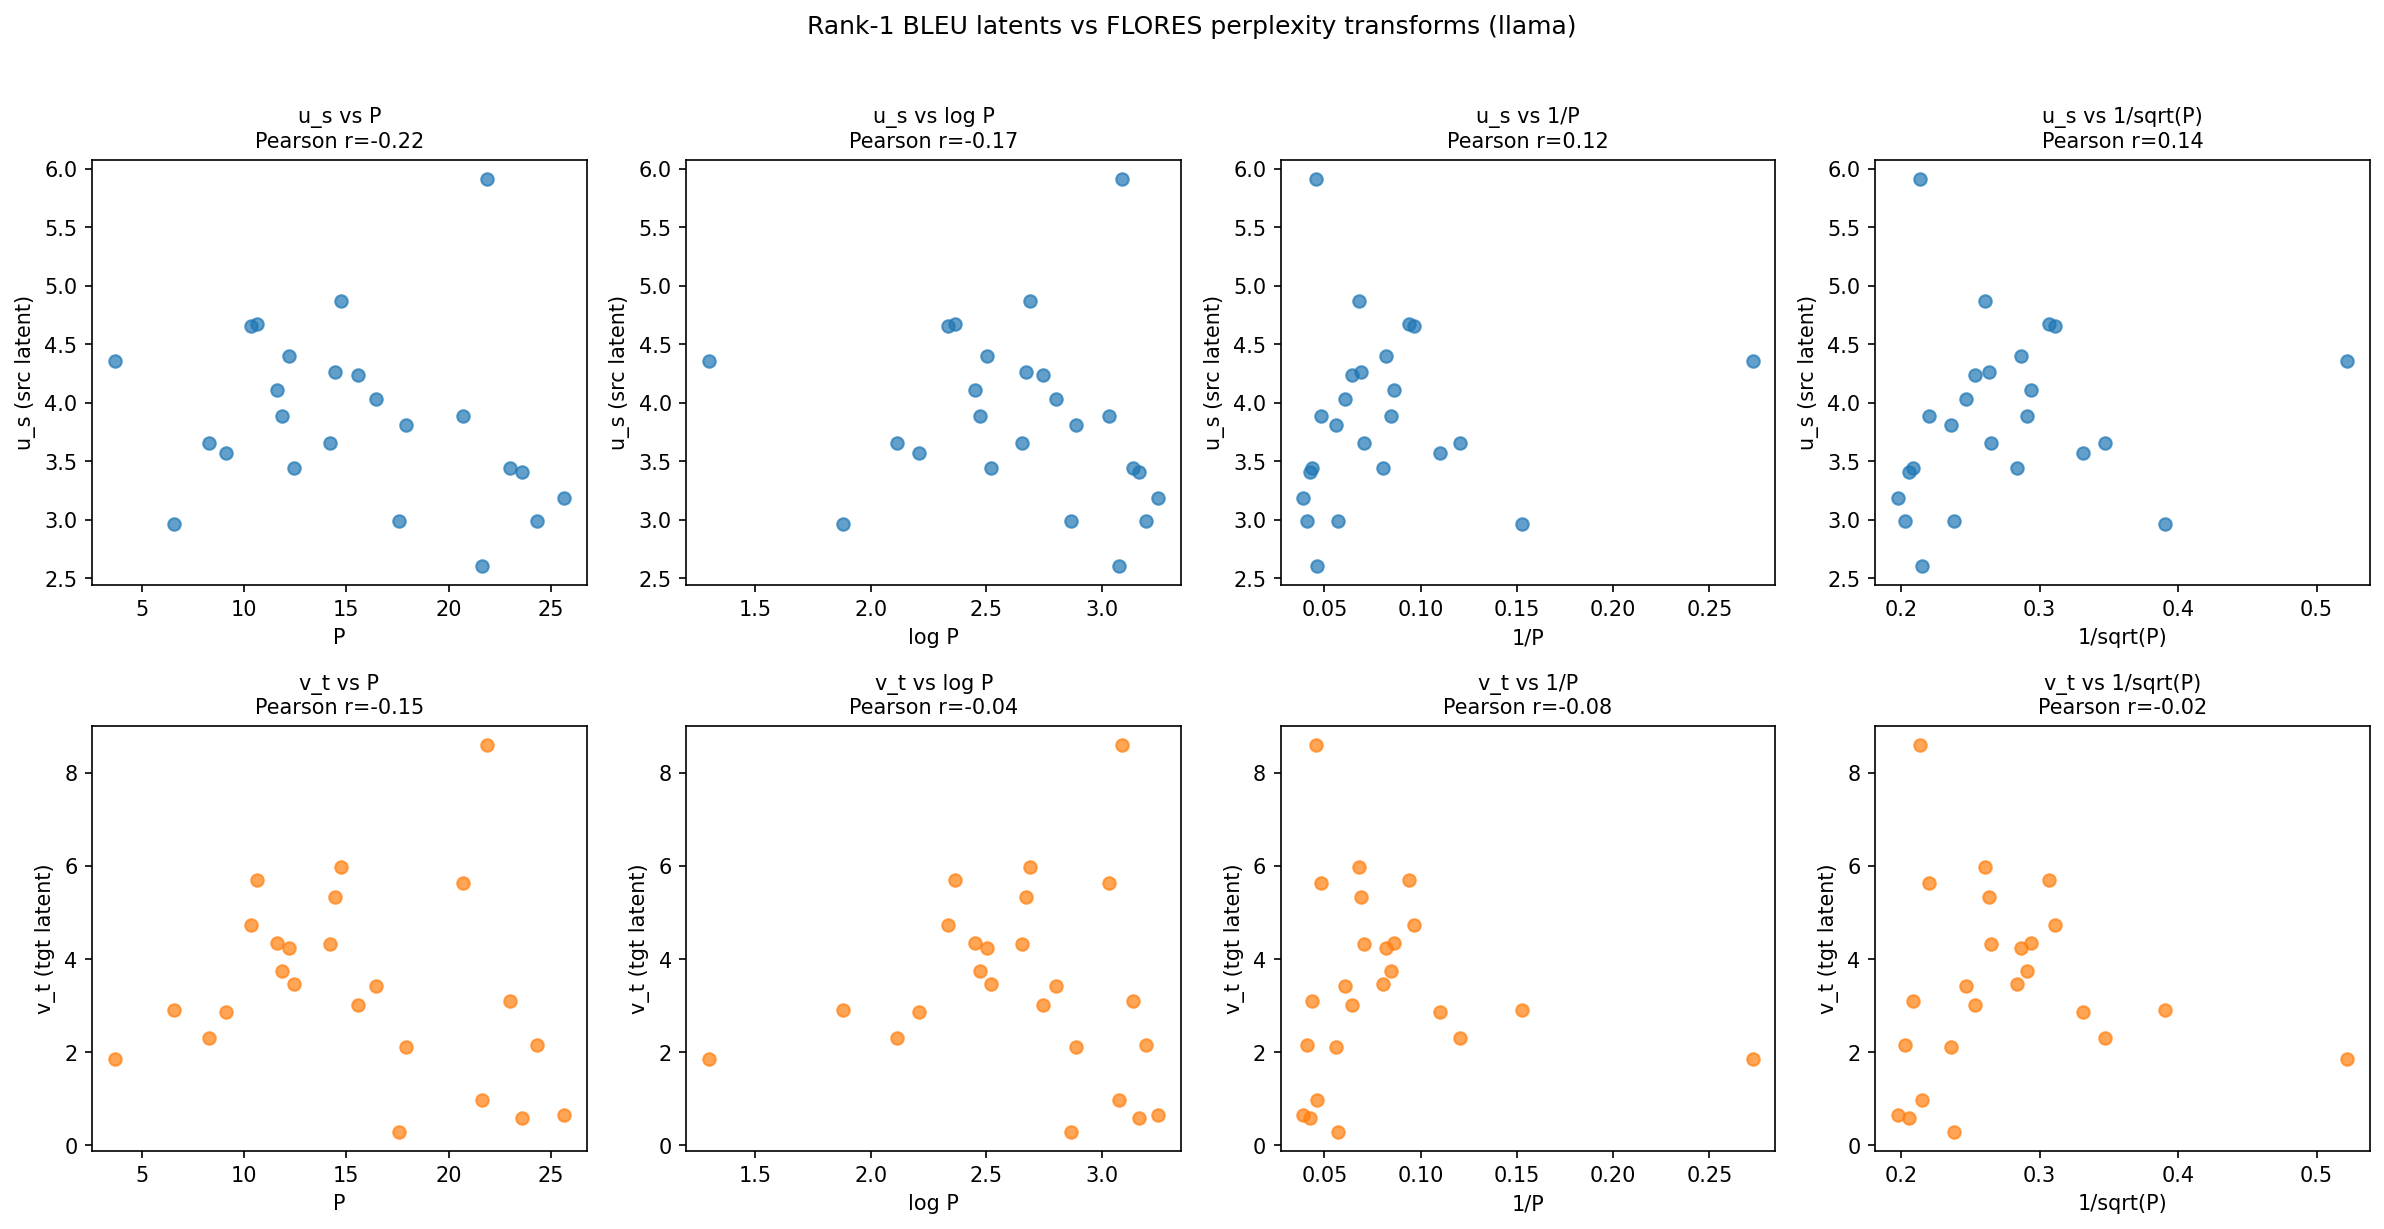
\includegraphics[width=0.95\linewidth]{../../img/perplexity_bleu_linear/rank1_latent_vs_ppl_llama.png}
\caption{Llama: rank-1 latents vs FLORES PPL transforms.}
\end{figure}

\begin{figure}[h]
\centering
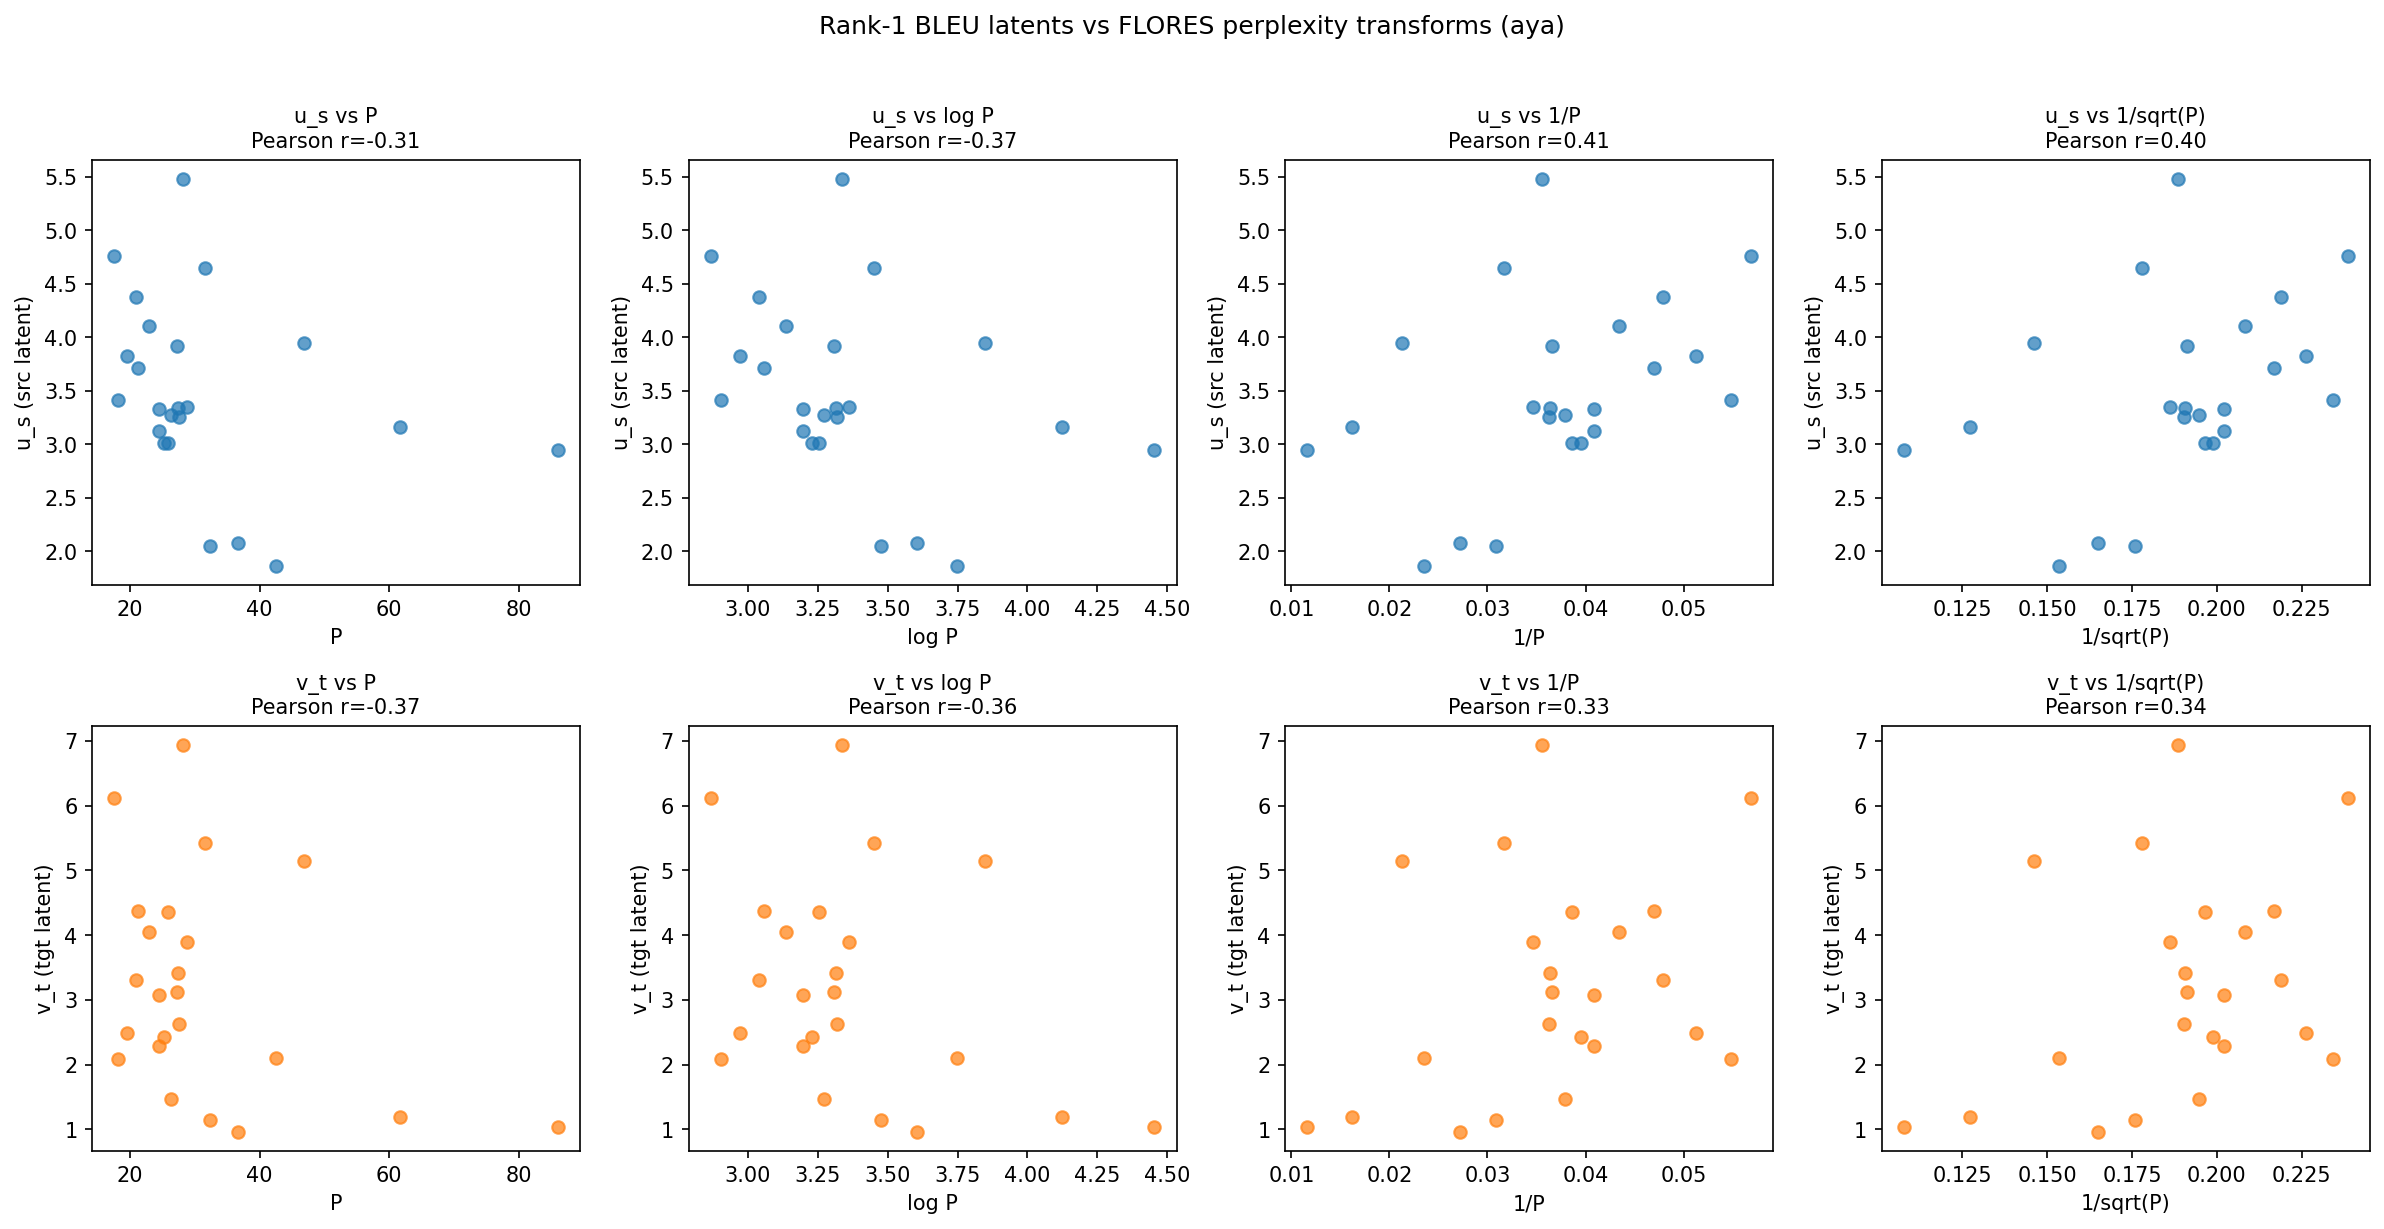
\includegraphics[width=0.95\linewidth]{../../img/perplexity_bleu_linear/rank1_latent_vs_ppl_aya.png}
\caption{Aya: rank-1 latents vs FLORES PPL transforms.}
\end{figure}

\section{Experiment 3: Log-multiplicative fit}

\subsection{Goal}

The rank-1 story is multiplicative ($\code{bleu} \approx u_s v_t$); the
natural \emph{linear} model in log space is therefore
\[
\log \code{bleu} = a + b \log \ppl_s + c \log \ppl_t + \varepsilon,
\quad\text{equivalently}\quad
\code{bleu} = e^a \cdot \ppl_s^{b} \cdot \ppl_t^{c}.
\]
Experiment 1 fit $\code{bleu}$ directly with an interaction; this fits the
right functional form for a multiplicative story. The question is how much
this functional change buys.

\subsection{Method}

Drop pairs with $\code{bleu} \le 0$ or missing PPL. Fit OLS in log space
per model. Report:

\begin{itemize}
  \item $R^2$ on the log scale (the scale we actually fit).
  \item $R^2$ on the BLEU scale (back-transformed predictions
    $\hat{y}_{\code{bleu}} = \exp(\hat{y}_{\log})$ vs actual BLEU). This is
    biased low by Jensen's inequality and is reported as a sanity check
    on practical utility, not as the model objective.
  \item $F$-test against intercept-only on the log scale.
  \item Per-coefficient $t$-tests.
\end{itemize}

\subsection{Results}

\begin{table}[h]
\centering
\small
\begin{tabular}{lrrrrrr}
\toprule
model & $n$ & $R^2_{\log}$ & $R^2_{\text{BLEU bt}}$ & $F(2,\text{df})$ & $p_F$ & coefs $(a,b,c)$ \\
\midrule
llama & 544 & 0.0421 & $-0.196$ & $11.89$ & $8.9\times10^{-6}$ &
  $(+3.48, -0.05, -0.38)$ \\
aya   & 505 & 0.1357 & $-0.002$ & $39.41$ & $1.3\times10^{-16}$ &
  $(+6.00, -0.39, -0.76)$ \\
\bottomrule
\end{tabular}
\caption{Log-multiplicative fit. Coefficients $b$ and $c$ are the exponents
on src and tgt PPL respectively in the back-transformed multiplicative
form.}
\end{table}

\paragraph{Per-coefficient significance:}

\begin{itemize}
  \item \textbf{Llama:} $b_{\log P_s} = -0.05$ ($p = 0.53$, n.s.); $c_{\log
    P_t} = -0.38$ ($p = 1.6\times10^{-6}$, highly significant).
  \item \textbf{Aya:} $b_{\log P_s} = -0.39$ ($p = 5.0\times10^{-5}$);
    $c_{\log P_t} = -0.76$ ($p = 5.8\times10^{-15}$). Both significant.
\end{itemize}

\subsection{Takeaways}

\begin{itemize}
  \item Switching to the right functional form (multiplicative in original
    scale, additive in log) does \emph{help}: Llama moves from $R^2 = 0.02$
    in raw space to $R^2_{\log} = 0.04$, and Aya moves from $0.10$ to
    $0.14$. The overall $F$-tests are highly significant.
  \item But: this is still nowhere near the rank-1 SVD's $88\%/82\%$.
    Consistent with Experiment 2 --- the issue is that $\log \ppl$ is a
    weak monotone signal for the underlying competence factor, not that
    the combination form is wrong.
  \item \textbf{Target perplexity carries most of the signal} in both
    models. For Llama, source PPL is essentially uninformative once tgt
    PPL is in the model. The src/tgt asymmetry shows up again, mirroring
    Experiment 2's finding that tgt latents are even less well-explained
    by tgt PPL than src latents are by src PPL.
  \item The negative back-transformed $R^2$ (especially Llama at $-0.20$)
    shows that the log-linear fit, when exponentiated, predicts BLEU
    \emph{worse} than the BLEU mean. Don't read the model as
    BLEU-predictive in raw units; it is a likelihood model in log space.
\end{itemize}

\paragraph{Outputs.}

\code{outputs/perplexity\_bleu\_linear/log\_multiplicative/fit\_summary.csv} \\
\code{outputs/perplexity\_bleu\_linear/log\_multiplicative/coefficients.csv} \\
\code{outputs/perplexity\_bleu\_linear/log\_multiplicative/predictions\_\{llama,aya\}.csv} \\
\code{img/perplexity\_bleu\_linear/log\_multiplicative\_\{llama,aya\}.png}

\begin{figure}[h]
\centering
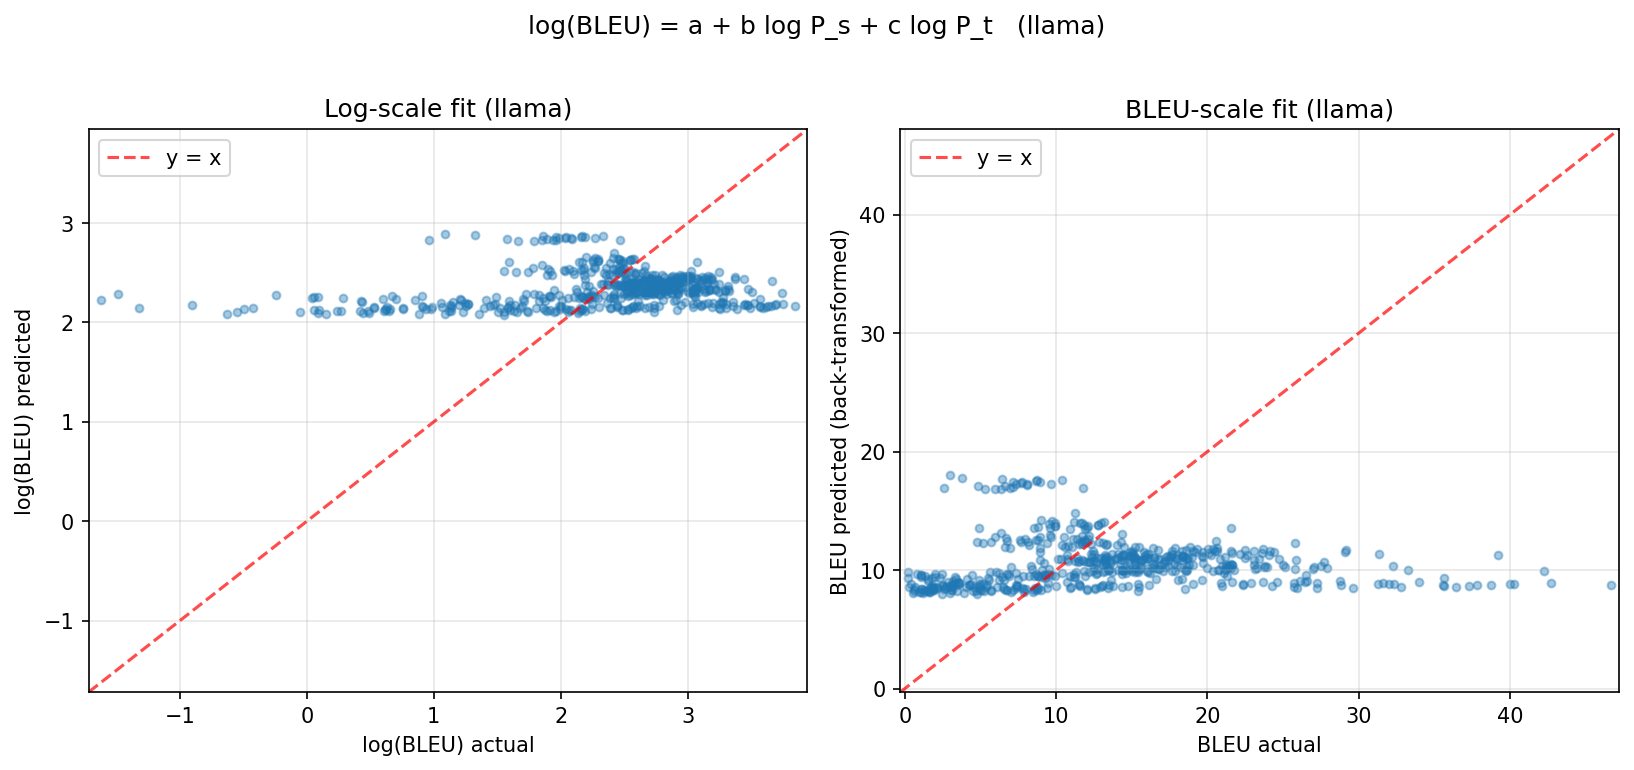
\includegraphics[width=0.95\linewidth]{../../img/perplexity_bleu_linear/log_multiplicative_llama.png}
\caption{Llama: log-multiplicative fit, log-scale (left) and back-transformed (right).}
\end{figure}

\begin{figure}[h]
\centering
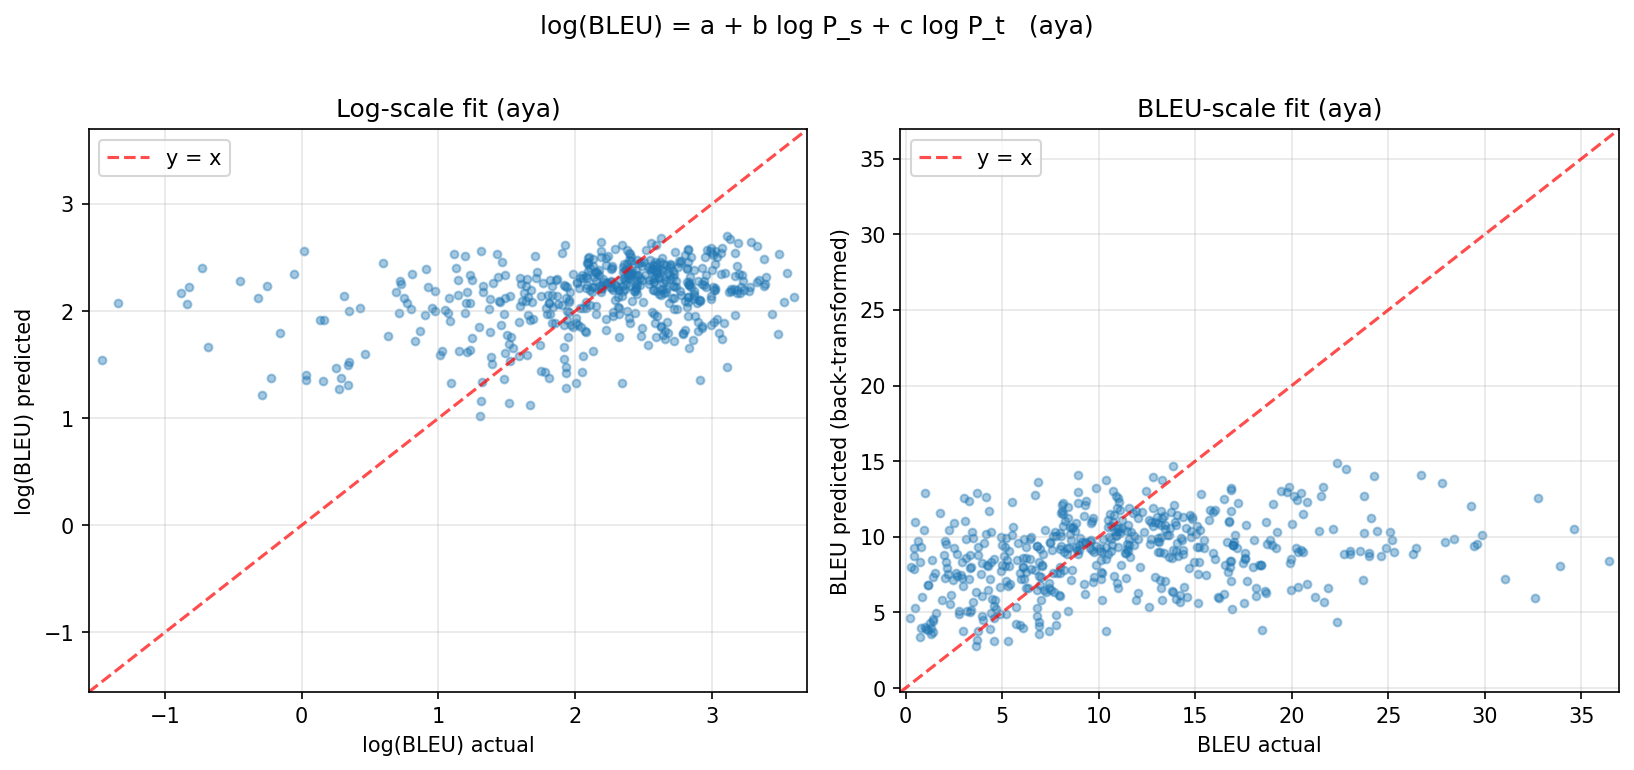
\includegraphics[width=0.95\linewidth]{../../img/perplexity_bleu_linear/log_multiplicative_aya.png}
\caption{Aya: log-multiplicative fit, log-scale (left) and back-transformed (right).}
\end{figure}

\section{Interim status after Experiments 1--3}

After three experiments, the empirical picture is:

\begin{enumerate}
  \item Linear-in-PPL with or without an $\ppl_s \cdot \ppl_t$ interaction:
    $R^2 \le 0.11$; interaction not significant (Experiment 1).
  \item Rank-1 BLEU latents correlate only weakly ($|\rho| \le 0.43$) with
    any tested monotone transform of FLORES PPL (Experiment 2).
  \item Log-multiplicative model is highly significant overall but captures
    at most $14\%$ of the log-BLEU variance (Experiment 3).
\end{enumerate}

This motivates the next batch: re-cast competence as the per-language
additive effects of a random-effects model, compare apples-to-apples
against the rank-1 SVD on a centered scale, repeat the PPL correlations
with language-labeled scatter plots, and unpack the src/tgt asymmetry that
appears across Experiments 2 and 3.

\section{Experiment 4: Additive RE model vs rank-1 SVD on a common scale}

\subsection{Goal}

Fit the additive random-effects-style model
\[
\code{bleu}_{ij} = \mu + \alpha_i + \beta_j + \varepsilon_{ij},
\]
estimate per-language $\alpha$ (src effect) and $\beta$ (tgt effect), and
compare to rank-1 SVD on a comparable scale.

\paragraph{On RE-model vs PCA.}

The additive RE model is \emph{not} identical to PCA/rank-1 SVD. RE is
\emph{additive}; rank-1 SVD is \emph{multiplicative}. They coincide only up
to a $\log$ transform: additive on $\log \code{bleu}$ $\approx$ rank-1 SVD on
$\code{bleu}$. Additive on raw BLEU is a separate model class.

A subtle but important detail: the original ``rank-1 faithfulness $= 88\%$''
metric is
\[
1 - \|M - M_1\|_F / \|M\|_F,
\]
measured against the \emph{uncentered} matrix norm. For Llama, $\sim 72\%$
of $\|M\|_F^2$ is the squared grand mean ($552 \cdot 13.27^2 \approx 97{,}166$
out of $\|M\|_F^2 \approx 135{,}297$), so the headline number is partly
inflated by the metric rather than reflecting only structural fit. We
report standard centered $R^2$ alongside it, and Section~\ref{sec:structural}
gives the apples-to-apples structural comparison between additive and
multiplicative model classes.

\subsection{Method}

Fit by OLS in long format with $\code{src}$ and $\code{tgt}$ dummies (drop
the last category on each side for identifiability; re-center coefficients
to sum to zero so $\mu$ is the grand mean and $\alpha, \beta$ are
deviations). Then evaluate four decompositions on the observed cells using
$R^2 = 1 - \mathrm{RSS}/\mathrm{TSS}_{\text{centered}}$:

\begin{itemize}
  \item Additive RE (47 parameters: $1 + 2(n_{\text{lang}}-1)$).
  \item Rank-1 SVD on uncentered $M$ (existing approach).
  \item Rank-1 SVD on centered $M$ (matches additive's centering).
  \item AMMI: additive $+$ rank-1 of the additive residuals.
\end{itemize}

\subsection{Results}

\begin{table}[h]
\centering
\small
\begin{tabular}{lrrrrrrr}
\toprule
model & $\bar y$ & SD & add & SVD($M$) & $\bar y + $SVD($M-\bar y$) & AMMI & faith.\ SVD \\
\midrule
llama & 13.27 & 8.32 & 0.932 & 0.960 & 0.859 & 0.965 & 0.894 \\
aya   & 10.81 & 6.77 & 0.879 & 0.899 & 0.716 & 0.925 & 0.832 \\
\bottomrule
\end{tabular}
\caption{First four model columns are standard centered $R^2 =
1 - \sum(y-\hat y)^2 / \sum(y-\bar y)^2$, on $n=552$ observed cells per
model. The final ``faith.\ SVD'' column is the original uncentered $1 -
\|M - M_1\|_F / \|M\|_F$ metric. The two SVD-based R² columns differ
substantively: column 4 (``SVD($M$)'') is the rank-1 SVD of the raw matrix
used as a predictor of BLEU; column 5 (``$\bar y + $SVD($M-\bar y$)'') is
the structurally honest comparison to the additive model -- both use the
grand mean as a constant offset and the rank-1 captures only the centered
residual. See Section~\ref{sec:structural}.}
\end{table}

\subsection{Takeaways}

\begin{itemize}
  \item The $88\%$ headline ``faithfulness'' is on an uncentered Frobenius
    scale where the squared grand mean dominates $\|M\|_F^2$ (Llama: $72\%$;
    Aya: $66\%$). On standard centered $R^2$, the same rank-1 SVD of
    uncentered $M$ achieves $0.960 / 0.899$ (Llama / Aya); the headline is
    not ``mostly the mean'', but the metric inflates it.
  \item The four R² columns measure different things. Comparing additive
    ($0.932 / 0.879$) to ``SVD$(M)$'' ($0.960 / 0.899$) is \emph{not} the
    structural ``additive vs multiplicative'' question, because the single
    rank-1 outer product is allowed to absorb the mean, the per-language
    main effects, \emph{and} multiplicative interaction all together. The
    apples-to-apples structural comparison is additive vs.
    ``$\bar y + $SVD($M - \bar y$)'' -- both with the grand mean as a
    constant offset, both estimating only per-language structure. That
    comparison and its interpretation live in
    Section~\ref{sec:structural}.
  \item AMMI (additive + rank-1 of additive residuals) lifts $R^2$ to
    $0.965 / 0.925$, only $3$--$5$ percentage points above additive. The
    genuinely multiplicative residual interaction in BLEU is small.
\end{itemize}

\paragraph{Outputs.}

\code{outputs/perplexity\_bleu\_linear/additive\_random\_effects/fit\_summary.csv} \\
\code{outputs/perplexity\_bleu\_linear/additive\_random\_effects/coefficients\_\{llama,aya\}.csv} \\
\code{outputs/perplexity\_bleu\_linear/additive\_random\_effects/bleu\_matrix\_\{llama,aya\}.csv}

\section{Experiment 5: Additive $\alpha,\beta$ effects vs FLORES PPL}

\subsection{Goal}

Repeat Experiment 2's correlation study with the additive-model
coefficients in place of the SVD vectors. The additive coefficients are
more directly interpretable as ``how much above/below the grand-mean BLEU
does this language tend to contribute as src / tgt''. Produce
language-labeled scatter plots to identify outlier languages.

\subsection{Results}

\begin{table}[h]
\centering
\small
\begin{tabular}{llrrrr}
\toprule
model & role & transform & Pearson $r$ & Pearson $p$ & Spearman $\rho$ \\
\midrule
\multirow{8}{*}{aya}
 & src ($\alpha$) & raw       & $-0.304$ & 0.158 & $-0.418$ \\
 & src ($\alpha$) & log       & $-0.362$ & 0.089 & $-0.418$ \\
 & src ($\alpha$) & $1/P$     & $+0.398$ & 0.060 & $+0.418$ \\
 & src ($\alpha$) & $1/\sqrt{P}$ & $+0.384$ & 0.071 & $+0.418$ \\
 & tgt ($\beta$)  & raw       & $-0.358$ & 0.094 & $-0.292$ \\
 & tgt ($\beta$)  & log       & $-0.344$ & 0.108 & $-0.292$ \\
 & tgt ($\beta$)  & $1/P$     & $+0.316$ & 0.142 & $+0.292$ \\
 & tgt ($\beta$)  & $1/\sqrt{P}$ & $+0.331$ & 0.123 & $+0.292$ \\
\midrule
\multirow{8}{*}{llama}
 & src ($\alpha$) & raw       & $-0.188$ & 0.378 & $-0.306$ \\
 & src ($\alpha$) & log       & $-0.141$ & 0.511 & $-0.306$ \\
 & src ($\alpha$) & $1/P$     & $+0.104$ & 0.630 & $+0.306$ \\
 & src ($\alpha$) & $1/\sqrt{P}$ & $+0.119$ & 0.579 & $+0.306$ \\
 & tgt ($\beta$)  & raw       & $-0.145$ & 0.500 & $-0.216$ \\
 & tgt ($\beta$)  & log       & $-0.037$ & 0.862 & $-0.216$ \\
 & tgt ($\beta$)  & $1/P$     & $-0.076$ & 0.724 & $+0.216$ \\
 & tgt ($\beta$)  & $1/\sqrt{P}$ & $-0.022$ & 0.917 & $+0.216$ \\
\bottomrule
\end{tabular}
\caption{Correlation between additive-model $\alpha, \beta$ and per-language
FLORES PPL. $n = 24$ per row. Compare to Experiment 2: numbers are nearly
identical, confirming that the additive coefficients and the rank-1 SVD
latents are estimating closely related per-language scalars (after
subtraction of the mean, which dominates the SVD).}
\end{table}

\subsection{Outlier languages (regress $\alpha$ or $\beta$ on $\log P$,
take largest signed residuals)}

\begin{itemize}
  \item \textbf{Llama, src ($\alpha$):} \code{eng} $(+8.47)$, \code{kor}
    $(-4.37)$, \code{hin} $(-4.28)$. English is far above its PPL-predicted
    src competence; Korean and Hindi are below.
  \item \textbf{Llama, tgt ($\beta$):} \code{eng} $(+21.07)$, \code{jpn}
    $(-12.15)$, \code{zho\_simpl} $(-10.68)$. English is a massive positive
    outlier as a target; Japanese and Chinese are massive negative outliers
    --- much lower BLEU as target than their FLORES PPL would predict.
    Tokenization on CJK is a known confound for BLEU.
  \item \textbf{Aya, src ($\alpha$):} \code{eng} $(+7.62)$, \code{jpn}
    $(-4.79)$, \code{tur} $(-4.14)$.
  \item \textbf{Aya, tgt ($\beta$):} \code{eng} $(+13.46)$, \code{ind}
    $(+9.58)$, \code{por} $(+8.33)$. All three are positive outliers;
    Indonesian and Portuguese ``over-deliver'' as targets relative to their
    PPL.
\end{itemize}

\paragraph{Implication.}

The PPL-vs-competence story is dominated by a small number of outlier
languages, especially English (always a positive outlier in magnitude) and
CJK targets in Llama (always a negative outlier). Removing English alone
would likely change the headline correlations substantially.

\paragraph{Outputs.}

\code{outputs/perplexity\_bleu\_linear/alpha\_beta\_vs\_ppl/correlations.csv} \\
\code{img/perplexity\_bleu\_linear/alpha\_beta\_vs\_ppl\_\{llama,aya\}.png}

\begin{figure}[h]
\centering
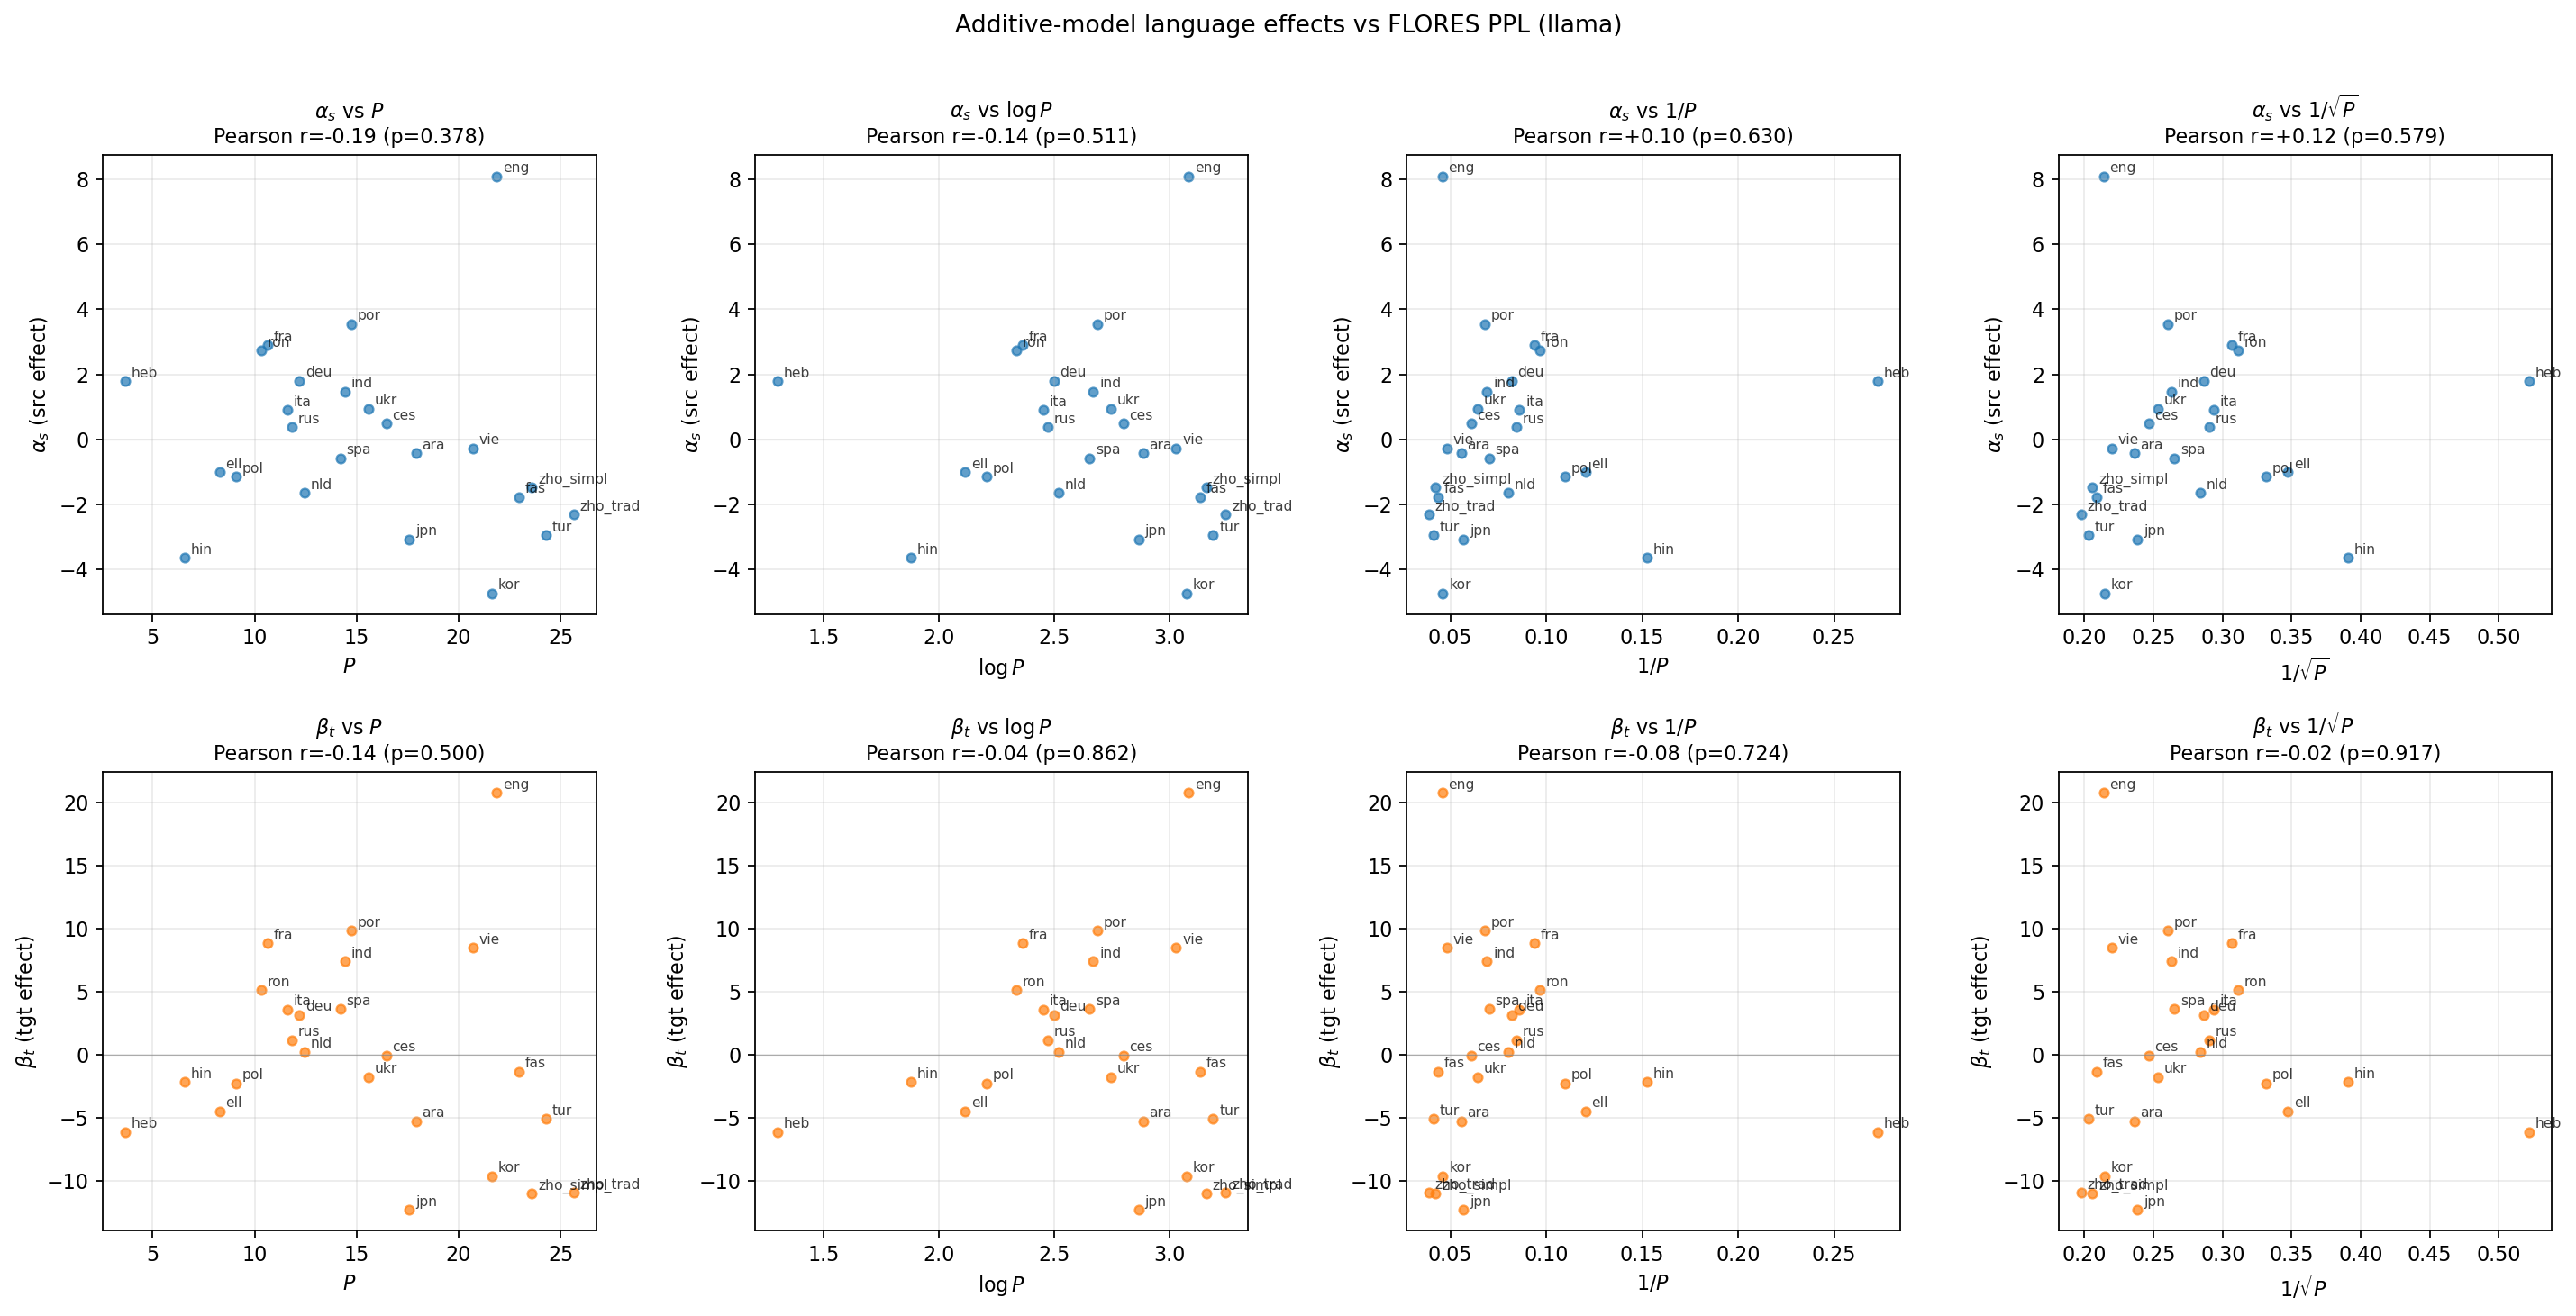
\includegraphics[width=0.95\linewidth]{../../img/perplexity_bleu_linear/alpha_beta_vs_ppl_llama.png}
\caption{Llama: additive $\alpha_s$ and $\beta_t$ vs FLORES PPL transforms,
labeled by language. English is a positive outlier; \code{jpn} and
\code{zho\_simpl} are far-negative as targets.}
\end{figure}

\begin{figure}[h]
\centering
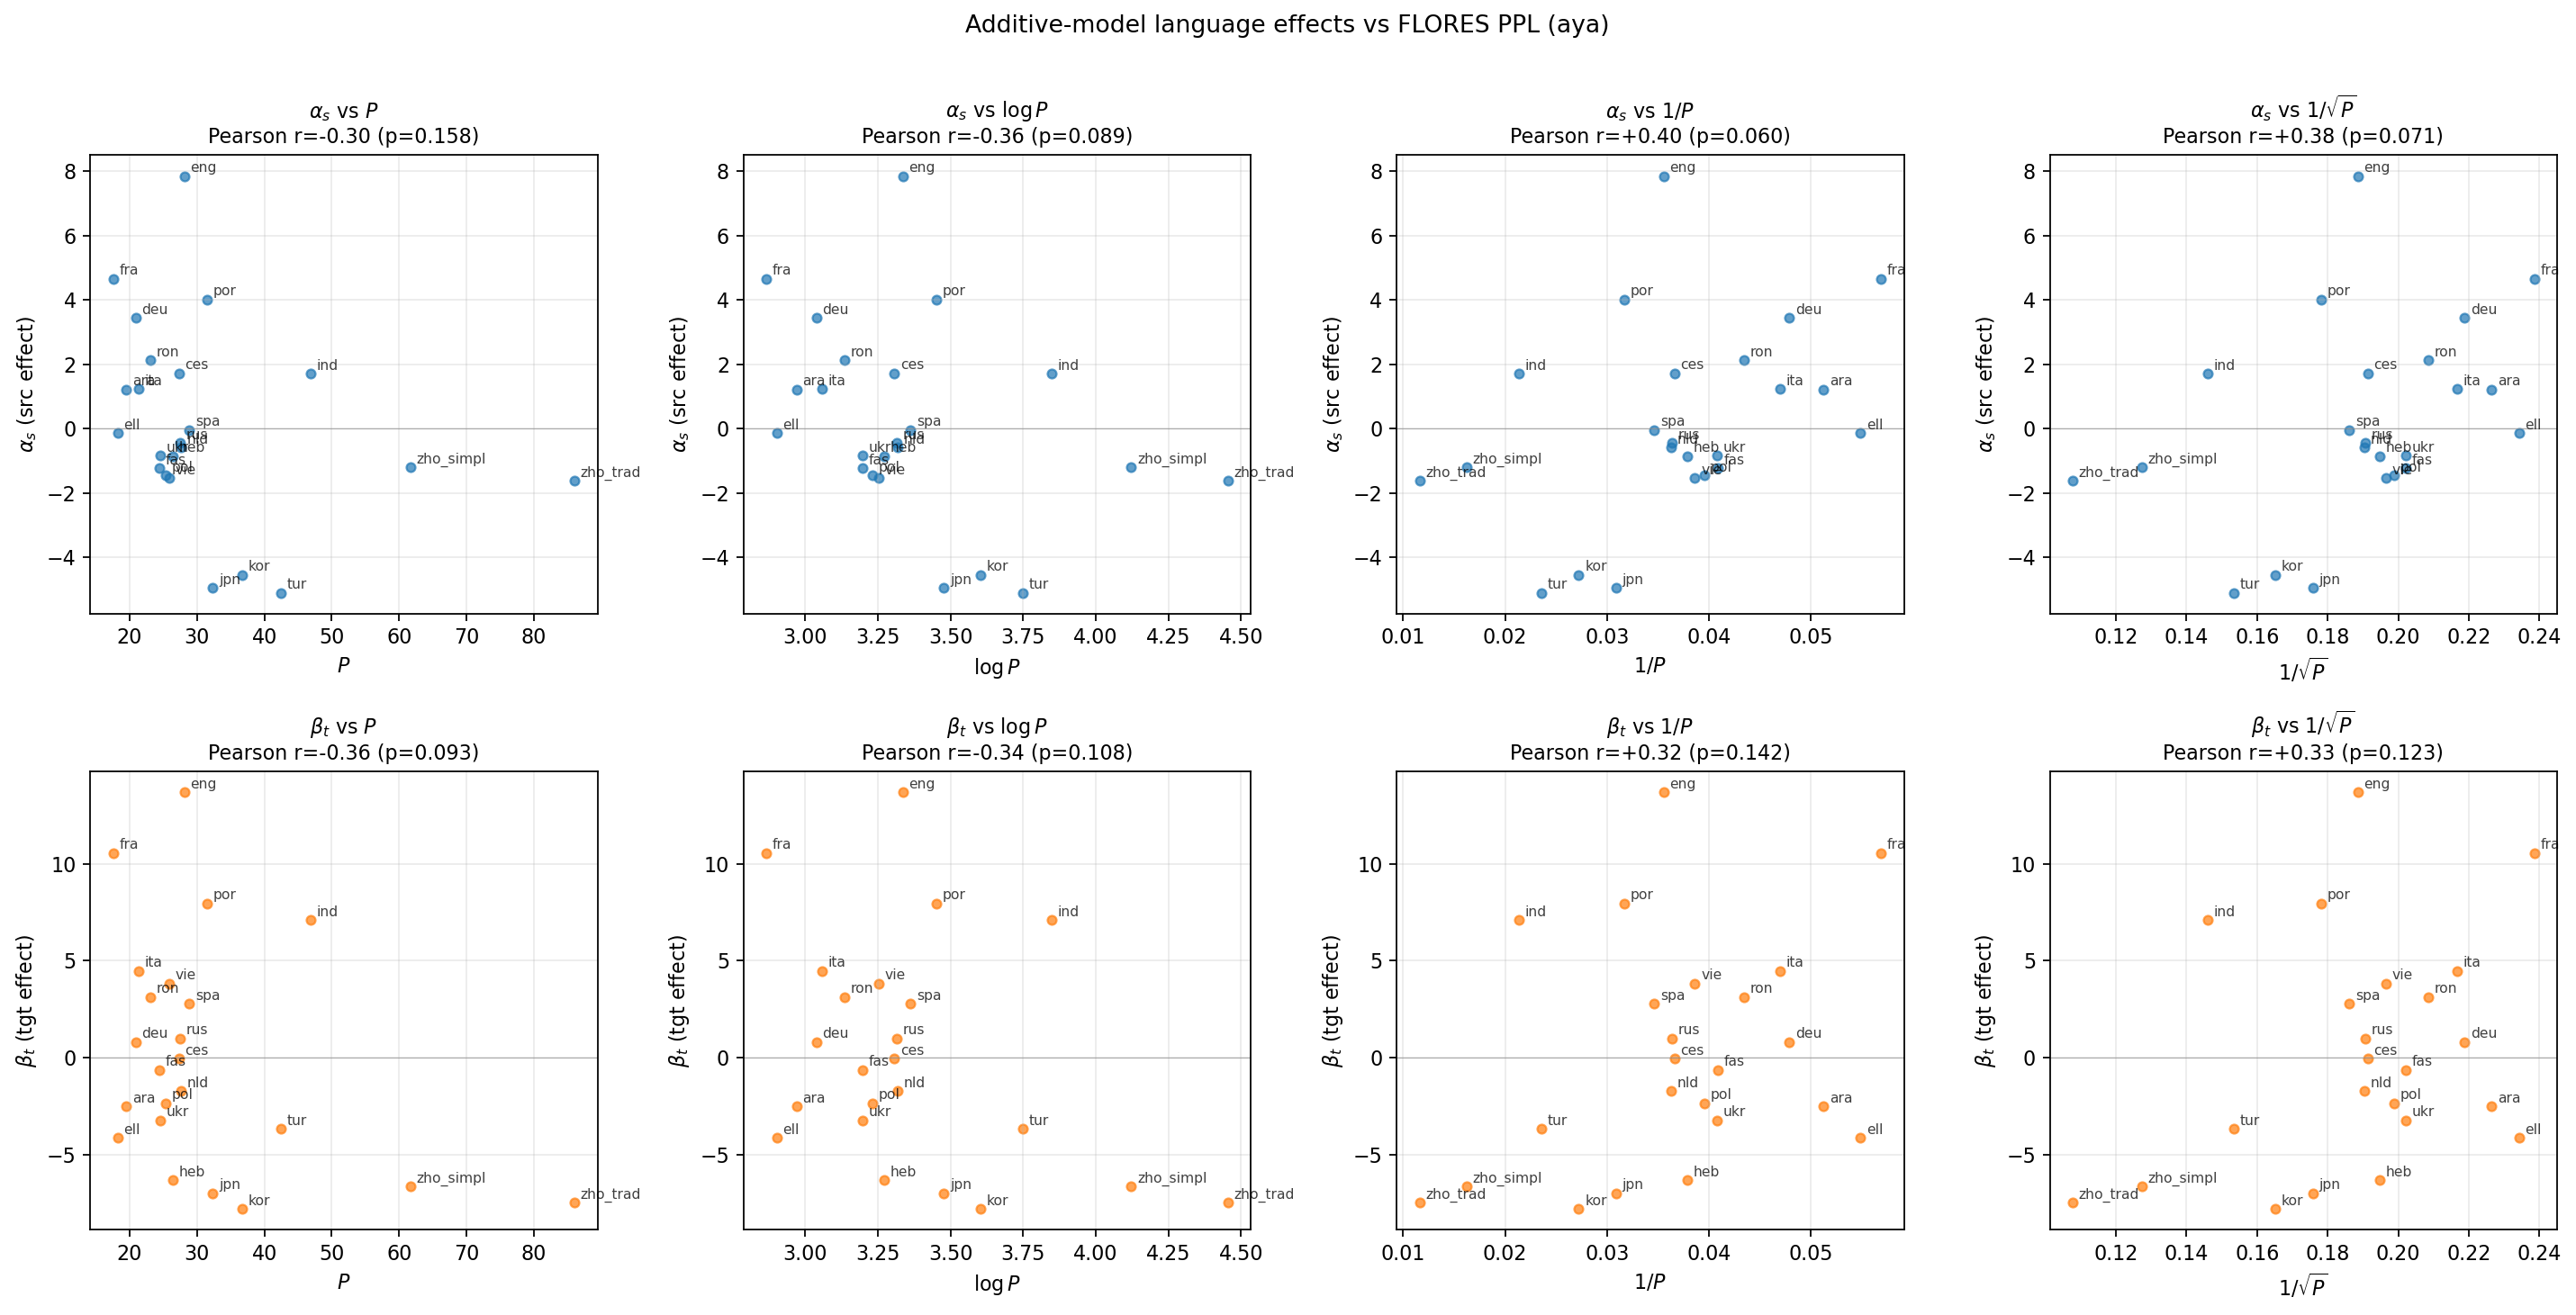
\includegraphics[width=0.95\linewidth]{../../img/perplexity_bleu_linear/alpha_beta_vs_ppl_aya.png}
\caption{Aya: additive $\alpha_s$ and $\beta_t$ vs FLORES PPL transforms,
labeled by language.}
\end{figure}

\section{Experiment 6: Why src signal $>$ tgt in Experiments 2/5 but
tgt signal $>$ src in Experiment 3?}

\subsection{The puzzle}

In Experiments 2 and 5 (per-language: $n=24$) the source-side Spearman
correlation with PPL is stronger than the target-side:
$|\rho_{\text{src}}| > |\rho_{\text{tgt}}|$ for both models. In
Experiment 3 (per-pair: $n \approx 550$) the target-side log-PPL coefficient
is much larger in absolute value than the source-side. These look like
opposing claims; they are not.

\subsection{Diagnostic results}

\paragraph{D1 --- Variance decomposition of BLEU across languages.}

\begin{center}
\small
\begin{tabular}{lrrr}
\toprule
model & var(mean BLEU as src) & var(mean BLEU as tgt) & ratio tgt/src \\
\midrule
llama & 6.11  & 56.62 & \textbf{9.26} \\
aya   & 7.66  & 32.69 & \textbf{4.27} \\
\bottomrule
\end{tabular}
\end{center}

Between-tgt-language BLEU variance is \textbf{4--9$\times$} larger than
between-src-language variance. Choosing a different target moves BLEU much
more than choosing a different source.

\paragraph{D6 --- Sequential ANOVA: how much $R^2$ does each side carry?}

\begin{center}
\small
\begin{tabular}{lrrrrr}
\toprule
model & $R^2$ src only & $R^2$ tgt only & $R^2$ additive both
      & marg.\ gain src$\mid$tgt & marg.\ gain tgt$\mid$src \\
\midrule
llama & 0.0911 & \textbf{0.8208} & 0.9307 & 0.1099 & \textbf{0.8396} \\
aya   & 0.1617 & \textbf{0.6889} & 0.8768 & 0.1880 & \textbf{0.7151} \\
\bottomrule
\end{tabular}
\end{center}

For Llama, tgt dummies \emph{alone} explain $82\%$ of BLEU variance; src
dummies alone explain only $9\%$. This is the structural reason a per-pair
regression places almost all the weight on tgt PPL: that is where almost
all of the BLEU variance lives.

\paragraph{D3/D5 --- Per-pair correlations.}

Per-pair univariate correlations on log scale:

\begin{center}
\small
\begin{tabular}{lrr}
\toprule
model & $r(\log B, \log P_s)$ & $r(\log B, \log P_t)$ \\
\midrule
llama & $-0.018$ & $-0.203$ \\
aya   & $-0.155$ & $-0.327$ \\
\bottomrule
\end{tabular}
\end{center}

Partial correlations (controlling for the other side):

\begin{center}
\small
\begin{tabular}{lrr}
\toprule
model & $r(\log B, \log P_s \mid \log P_t)$ & $r(\log B, \log P_t \mid \log P_s)$ \\
\midrule
llama & $-0.027$ & $-0.204$ \\
aya   & $-0.180$ & $-0.338$ \\
\bottomrule
\end{tabular}
\end{center}

Univariate and partial correlations are essentially equal --- $\log P_s$
and $\log P_t$ are nearly uncorrelated in the per-pair design (as they
must be, given a balanced full-grid of language pairs). So the
``tgt-dominant'' coefficient in Experiment 3 is not a multicollinearity
artifact.

\paragraph{D2 --- Per-language correlations of mean BLEU with PPL.}

\begin{center}
\small
\begin{tabular}{lrrrr}
\toprule
model & $r(\bar B_{\text{as-src}}, \log P_s)$ & Spearman & $r(\bar B_{\text{as-tgt}}, \log P_t)$ & Spearman \\
\midrule
llama & $-0.172$ & $-0.327$ & $-0.034$ & $-0.216$ \\
aya   & $-0.359$ & $-0.438$ & $-0.342$ & $-0.295$ \\
\bottomrule
\end{tabular}
\end{center}

Once we collapse to per-language scalars, src and tgt look closer. Llama
target is essentially uncorrelated with $\log P_t$ in Pearson (driven by
the Japanese/Chinese outliers identified in Experiment 5).

\subsection{Resolution}

The two views measure orthogonal things:

\begin{itemize}
  \item \textbf{Per-pair regression (Exp 3)} asks ``how much BLEU
    variation does $\log P$ explain?'' The answer is dominated by which
    side has more BLEU variation to explain. tgt has $4$--$9\times$ the
    between-language variance of src (D1), so even at the same per-language
    correlation strength, tgt PPL has more to ``soak up'' and its
    regression coefficient is larger and more significant.
  \item \textbf{Per-language correlation (Exp 2 / 5)} asks ``how
    well-ordered are the languages by PPL?'' This is scale-invariant: it
    does not care how much BLEU variance is on each axis, only whether the
    \emph{ranks} of languages line up. Here, tgt is hurt by a few large
    outliers (\code{jpn}, \code{zho\_simpl} for Llama --- see Experiment 5)
    that drag the correlation down, while src is more uniform.
\end{itemize}

So both observations are correct and compatible: \textbf{tgt is the
high-leverage axis} for BLEU prediction, but \textbf{src has the cleaner
per-language PPL signal} once we strip out scale and look only at ordering.

\section{Experiment 7: Apples-to-apples additive vs multiplicative
(subtracting the grand mean)}
\label{sec:structural}

\subsection{Why subtract the grand mean}

The BLEU matrix has a large positive grand mean ($\bar y \approx 13$ for
Llama, $\approx 11$ for Aya). Any model with a free intercept or constant
offset captures this trivially. The Frobenius faithfulness metric
\[
1 - \|M - M_1\|_F / \|M\|_F
\]
used in the original ``$88\%$'' claim is measured against the uncentered
$\|M\|_F$, where the squared grand mean accounts for $\sim 72\%$ of the
denominator (Llama). So that headline metric does \emph{not} cleanly
distinguish ``rank-1 captures the mean'' from ``rank-1 captures
per-language structure''.

To compare model classes \emph{structurally} -- additive main effects vs.
multiplicative interaction -- we put both on equal footing:

\begin{itemize}
  \item Both models are given the grand mean as a fixed constant offset
    (not credited as ``explained'' by the model).
  \item Each model estimates per-language structure with a comparable
    parameter budget.
  \item Performance is measured on \emph{centered} variance,
    $R^2 = 1 - \sum(y - \hat y)^2 / \sum(y - \bar y)^2$. The denominator
    already subtracts $\bar y$, so neither model is rewarded for matching it.
\end{itemize}

Equivalently: in OLS the additive model satisfies $\hat\mu = \bar y$
exactly, so fitting $\mu + \alpha + \beta$ to $M$ is the same as fitting
$\alpha + \beta$ to $(M - \bar y)$. Doing the analogous mean subtraction
for the rank-1 model gives the structurally honest comparison.

\subsection{Model specifications}

\begin{center}
\small
\begin{tabular}{lll}
\toprule
model & functional form & per-lang free parameters \\
\midrule
additive (RE)   & $\hat y_{ij} = \bar y + \alpha_i + \beta_j$              & $2(n-1) = 46$ \\
multiplicative  & $\hat y_{ij} = \bar y + u_i v_j$                         & $2n - 1 = 47$ \\
AMMI            & $\hat y_{ij} = \bar y + \alpha_i + \beta_j + u_i v_j$    & $\sim 93$ \\
\bottomrule
\end{tabular}
\end{center}

For additive, $\alpha$ and $\beta$ are sum-to-zero. For multiplicative,
$u v^T$ is the rank-1 SVD of $(M - \bar y)$, then added back to $\bar y$
at prediction time. AMMI nests additive: the rank-1 of additive
\emph{residuals} is the additional term. Parameter budgets per language
are essentially equal for additive and multiplicative ($46$ vs $47$);
AMMI has roughly twice as many.

\subsection{Results}

\begin{table}[h]
\centering
\small
\begin{tabular}{lcc}
\toprule
model & Llama $R^2_{\text{centered}}$ & Aya $R^2_{\text{centered}}$ \\
\midrule
intercept only ($\hat y = \bar y$)               & $0.000$ & $0.000$ \\
multiplicative ($\bar y + $rank-1 of $M - \bar y$) & $0.859$ & $0.716$ \\
additive ($\bar y + \alpha + \beta$)              & $\mathbf{0.932}$ & $\mathbf{0.879}$ \\
AMMI (additive $+$ rank-1 of additive residuals)  & $0.965$ & $0.925$ \\
\bottomrule
\end{tabular}
\caption{Centered $R^2$ for like-for-like comparisons. Both single-structure
models share the grand mean as a constant offset and have comparable
parameter budgets ($46$ vs $47$); they differ only in functional form.}
\end{table}

\subsection{Interpretation}

\begin{enumerate}
  \item \textbf{Additive wins the structural comparison.} With essentially
    equal per-language parameter budgets and the grand mean given to both,
    the additive model explains substantially more centered BLEU variance
    than multiplicative: $0.93$ vs $0.86$ for Llama ($+7$ pp), $0.88$ vs
    $0.72$ for Aya ($+16$ pp). The advantage is larger for Aya, consistent
    with Aya's BLEU matrix being less dominated by a single axis: in
    Experiment~6 the between-language variance ratio tgt:src was $9.3$ for
    Llama vs $4.3$ for Aya. A rank-1 outer product can absorb one dominant
    axis well; when both src and tgt axes carry comparable structure, it
    cannot fit them both.

  \item \textbf{Multiplicative is not vacuous.} $R^2 = 0.86 / 0.72$ is far
    from zero. For Llama specifically, the centered BLEU matrix is
    dominated by target main effects ($\beta$), which a single outer
    product can approximate fairly well -- this is why the multiplicative
    R² is high for Llama despite an additive matrix structure. The rank-1
    fit is mostly capturing $\beta$ projected through one outer product,
    not genuine multiplicative interaction.

  \item \textbf{AMMI shows multiplicative residual interaction is small.}
    Adding rank-1 of the additive residuals on top of the additive model
    lifts $R^2$ only $+3.3$ pp for Llama ($0.932 \to 0.965$) and $+4.6$ pp
    for Aya ($0.879 \to 0.925$). This is the magnitude of \emph{genuinely}
    multiplicative interaction, above and beyond additive main effects.
    It is real but small. Most of BLEU's per-language structure is
    additive; only a thin slice is multiplicative-on-top.

  \item \textbf{Reframing the $88\%$ headline.} The original ``rank-1 SVD
    is $88\%$ faithful'' claim was on the uncentered Frobenius scale and is
    inflated by the matrix's grand mean. The structurally precise statement,
    on a like-for-like scale, is: \emph{BLEU's per-language structure is
    dominantly additive ($93\%/88\%$), with a small multiplicative residual
    on top ($+3$--$5$ pp)}. ``H1 holds'' in the sense that BLEU does factor
    cleanly into per-language source and target competence; the
    factorization is additive rather than multiplicative.
\end{enumerate}

\paragraph{Note on rank-1 of uncentered $M$.} For completeness: a model
$\hat y_{ij} = (u v^T)_{ij}$ with no constant offset, fit by rank-1 SVD of
the raw matrix $M$, reaches centered $R^2 = 0.960 / 0.899$ -- slightly
above additive. This is \emph{not} a contradiction with point 1. That
single outer product is doing triple duty: capturing mean structure,
per-language deviations, and any interaction, all packed into one
$u v^T$. It is a perfectly legitimate model, but it is not a structural
``multiplicative'' model in the sense of ``deviation from the mean is
$u \cdot v$'' -- it lets rank-1 implicitly absorb additive main-effects
structure into its outer product. The like-for-like comparison above is
the one that answers the structural question.

\section{Experiment 8: Drop-English ablation --- outlier-driven vs systematic PPL signal}

\subsection{Goal}

Experiment 5 flagged English as the single largest positive outlier in
both $\alpha$ (src effect) and $\beta$ (tgt effect): $\alpha_{\text{eng}}
= +8.5$ (Llama) / $+7.6$ (Aya), $\beta_{\text{eng}} = +21.1$ (Llama) /
$+13.5$ (Aya) measured as signed residuals to the log-PPL trendline.
With $n = 24$, a single high-leverage point can dominate Pearson
correlations. The question: how much of Experiment 5's weak $\alpha,
\beta$ vs PPL signal is English-driven, and how much is systematic
across the other 23 languages?

\subsection{Method}

\begin{enumerate}
  \item Drop all pairs where $\code{src} = \code{eng}$ or $\code{tgt} =
    \code{eng}$ from \code{pair\_metrics.csv}: $552 \to 506$ pairs
    ($23 \times 22$).
  \item Refit the additive RE model on this reduced grid; recover new
    $\alpha$ and $\beta$ over $23$ languages.
  \item Compute Pearson and Spearman correlations of new $\alpha, \beta$
    against the same four PPL transforms used in Experiment 5
    (\code{raw}, $\log$, $1/P$, $1/\sqrt{P}$).
  \item Compare side-by-side with the full 24-lang correlations.
  \item Produce annotated scatter plots over the 23-lang set.
\end{enumerate}

\subsection{Structural fit unchanged}

The additive R² is essentially identical after dropping English:

\begin{center}
\small
\begin{tabular}{lrrr}
\toprule
model & $R^2$ (24 langs) & $R^2$ (23 langs, no eng) & $\Delta$ \\
\midrule
llama & 0.932 & 0.927 & $-0.005$ \\
aya   & 0.879 & 0.862 & $-0.017$ \\
\bottomrule
\end{tabular}
\end{center}

The grand mean drops slightly ($\bar y$ Llama $13.27 \to 12.02$, Aya
$10.81 \to 9.88$) as expected when removing English's high-BLEU rows
and columns, but the per-language additive structure still explains
$\sim 90\%$ of centered BLEU variance. So removing English doesn't
change the structural story of Section~\ref{sec:structural}.

\subsection{PPL correlations: side-by-side comparison}

\begin{table}[h]
\centering
\small
\begin{tabular}{llrrr|rrr}
\toprule
 & & \multicolumn{3}{c|}{Pearson $r$} & \multicolumn{3}{c}{Spearman $\rho$} \\
model & transform & full (24) & no eng (23) & $\Delta |r|$ & full & no eng & $\Delta |\rho|$ \\
\midrule
\multicolumn{8}{l}{\textbf{src ($\alpha$)}} \\
llama & raw       & $-0.188$ & $\mathbf{-0.441^*}$ & $+0.252$ & $-0.306$ & $-0.453$ & $+0.147$ \\
llama & log       & $-0.141$ & $-0.357$ & $+0.216$ & $-0.306$ & $-0.453$ & $+0.147$ \\
llama & $1/P$     & $+0.104$ & $+0.264$ & $+0.160$ & $+0.306$ & $+0.453$ & $+0.147$ \\
llama & $1/\sqrt{P}$ & $+0.119$ & $+0.308$ & $+0.189$ & $+0.306$ & $+0.453$ & $+0.147$ \\
aya   & raw       & $-0.304$ & $-0.310$ & $+0.006$ & $-0.418$ & $-0.444$ & $+0.026$ \\
aya   & log       & $-0.362$ & $-0.404$ & $+0.041$ & $-0.418$ & $-0.444$ & $+0.026$ \\
aya   & $1/P$     & $+0.398$ & $\mathbf{+0.476^*}$ & $+0.078$ & $+0.418$ & $+0.444$ & $+0.026$ \\
aya   & $1/\sqrt{P}$ & $+0.384$ & $\mathbf{+0.444^*}$ & $+0.060$ & $+0.418$ & $+0.444$ & $+0.026$ \\
\midrule
\multicolumn{8}{l}{\textbf{tgt ($\beta$)}} \\
llama & raw       & $-0.145$ & $-0.343$ & $+0.198$ & $-0.216$ & $-0.308$ & $+0.091$ \\
llama & log       & $-0.037$ & $-0.189$ & $+0.151$ & $-0.216$ & $-0.308$ & $+0.091$ \\
llama & $1/P$     & $-0.076$ & $+0.009$ & $-0.067$ & $+0.216$ & $+0.308$ & $+0.091$ \\
llama & $1/\sqrt{P}$ & $-0.022$ & $+0.096$ & $+0.074$ & $+0.216$ & $+0.308$ & $+0.091$ \\
aya   & raw       & $-0.358$ & $-0.390$ & $+0.032$ & $-0.292$ & $-0.340$ & $+0.048$ \\
aya   & log       & $-0.344$ & $-0.389$ & $+0.046$ & $-0.292$ & $-0.340$ & $+0.048$ \\
aya   & $1/P$     & $+0.316$ & $+0.378$ & $+0.062$ & $+0.292$ & $+0.340$ & $+0.048$ \\
aya   & $1/\sqrt{P}$ & $+0.331$ & $+0.385$ & $+0.054$ & $+0.292$ & $+0.340$ & $+0.048$ \\
\bottomrule
\end{tabular}
\caption{Correlation of additive $\alpha, \beta$ with FLORES PPL
transforms, full 24-lang set vs.\ 23-lang set after dropping English.
$\Delta |r|$ = $|r_{\text{no eng}}| - |r_{\text{full}}|$ (positive
$\Rightarrow$ stronger correlation after removing English). Bold
$^*$ marks $p < 0.05$ in the no-eng column.}
\end{table}

\subsection{Observations}

\begin{itemize}
  \item \textbf{Llama: English was suppressing most of the signal.}
    Pearson $|r|$ \emph{roughly doubles} on both src and tgt after
    removing English. Llama src raw $|r|$ goes $0.19 \to 0.44$;
    Llama tgt raw $|r|$ goes $0.15 \to 0.34$. Llama src raw is now
    statistically significant ($p = 0.035$).
  \item \textbf{Aya: signal is systematic, not English-driven.} Pearson
    $|r|$ changes by only $0$--$8$ pp after removing English. The
    correlation was already $\sim 0.4$ and stays at $\sim 0.4$. Aya src
    $1/P$ and $1/\sqrt{P}$ cross the $p < 0.05$ threshold, but the
    magnitude shift is small.
  \item \textbf{Spearman is robust either way.} Spearman shifts much
    less than Pearson when English is removed --- the rank structure
    was less affected by the single outlier than the Pearson magnitudes
    were. The gap between Spearman ($\sim 0.45$ src for both models)
    and Pearson on the full set therefore measures how much one outlier
    was distorting Pearson.
  \item \textbf{After removing English, the two models look similar.}
    Both have $|r|$ in the $0.3$--$0.45$ range for the best transforms,
    with Aya slightly stronger. The original ``Aya much better than
    Llama'' verdict from Experiments 2/5 was, for Llama in particular,
    a Pearson-vs-outlier artifact.
  \item \textbf{Best transforms (no eng).} Llama src: \code{raw}
    ($r = -0.44$). Aya src: $1/P$ ($r = +0.48$). Both directions
    correct (higher PPL $\to$ lower $\alpha$ src effect). Transforms
    differ slightly between models but all are monotone negative in $P$.
\end{itemize}

\subsection{Conclusion}

The Experiment 5 narrative ``FLORES PPL barely correlates with
per-language competence'' was substantially overstated for Llama. Once
English (a high-leverage positive outlier on both src and tgt sides) is
removed, the remaining 23 languages show systematic, moderate, and
statistically detectable correlations in the expected direction
($|r| \approx 0.35$--$0.45$, $|\rho| \approx 0.31$--$0.45$).

The PPL signal is therefore best described as \textbf{moderate and
systematic across non-English languages, with English as a strong
positive outlier} that obscures the signal in the full sample. This is
consistent with English being heavily over-represented in training
data: it has unusually good translation quality \emph{for its
perplexity}, breaking the monotonic PPL$\to$competence relationship.

A natural follow-up: drop the next-largest outliers (\code{jpn},
\code{zho\_simpl} for Llama tgt) and see if correlations strengthen
further --- or test with bootstrap resampling whether the remaining
$\sim 0.4$ correlations would have been detectable at $n = 23$
regardless.

\paragraph{Outputs.}

\code{outputs/perplexity\_bleu\_linear/drop\_english\_ablation/correlations\_no\_eng.csv} \\
\code{outputs/perplexity\_bleu\_linear/drop\_english\_ablation/comparison\_with\_full.csv} \\
\code{outputs/perplexity\_bleu\_linear/drop\_english\_ablation/coefficients\_no\_eng\_\{llama,aya\}.csv} \\
\code{outputs/perplexity\_bleu\_linear/drop\_english\_ablation/fit\_summary\_no\_eng.csv} \\
\code{img/perplexity\_bleu\_linear/alpha\_beta\_vs\_ppl\_no\_eng\_\{llama,aya\}.png}

\begin{figure}[h]
\centering
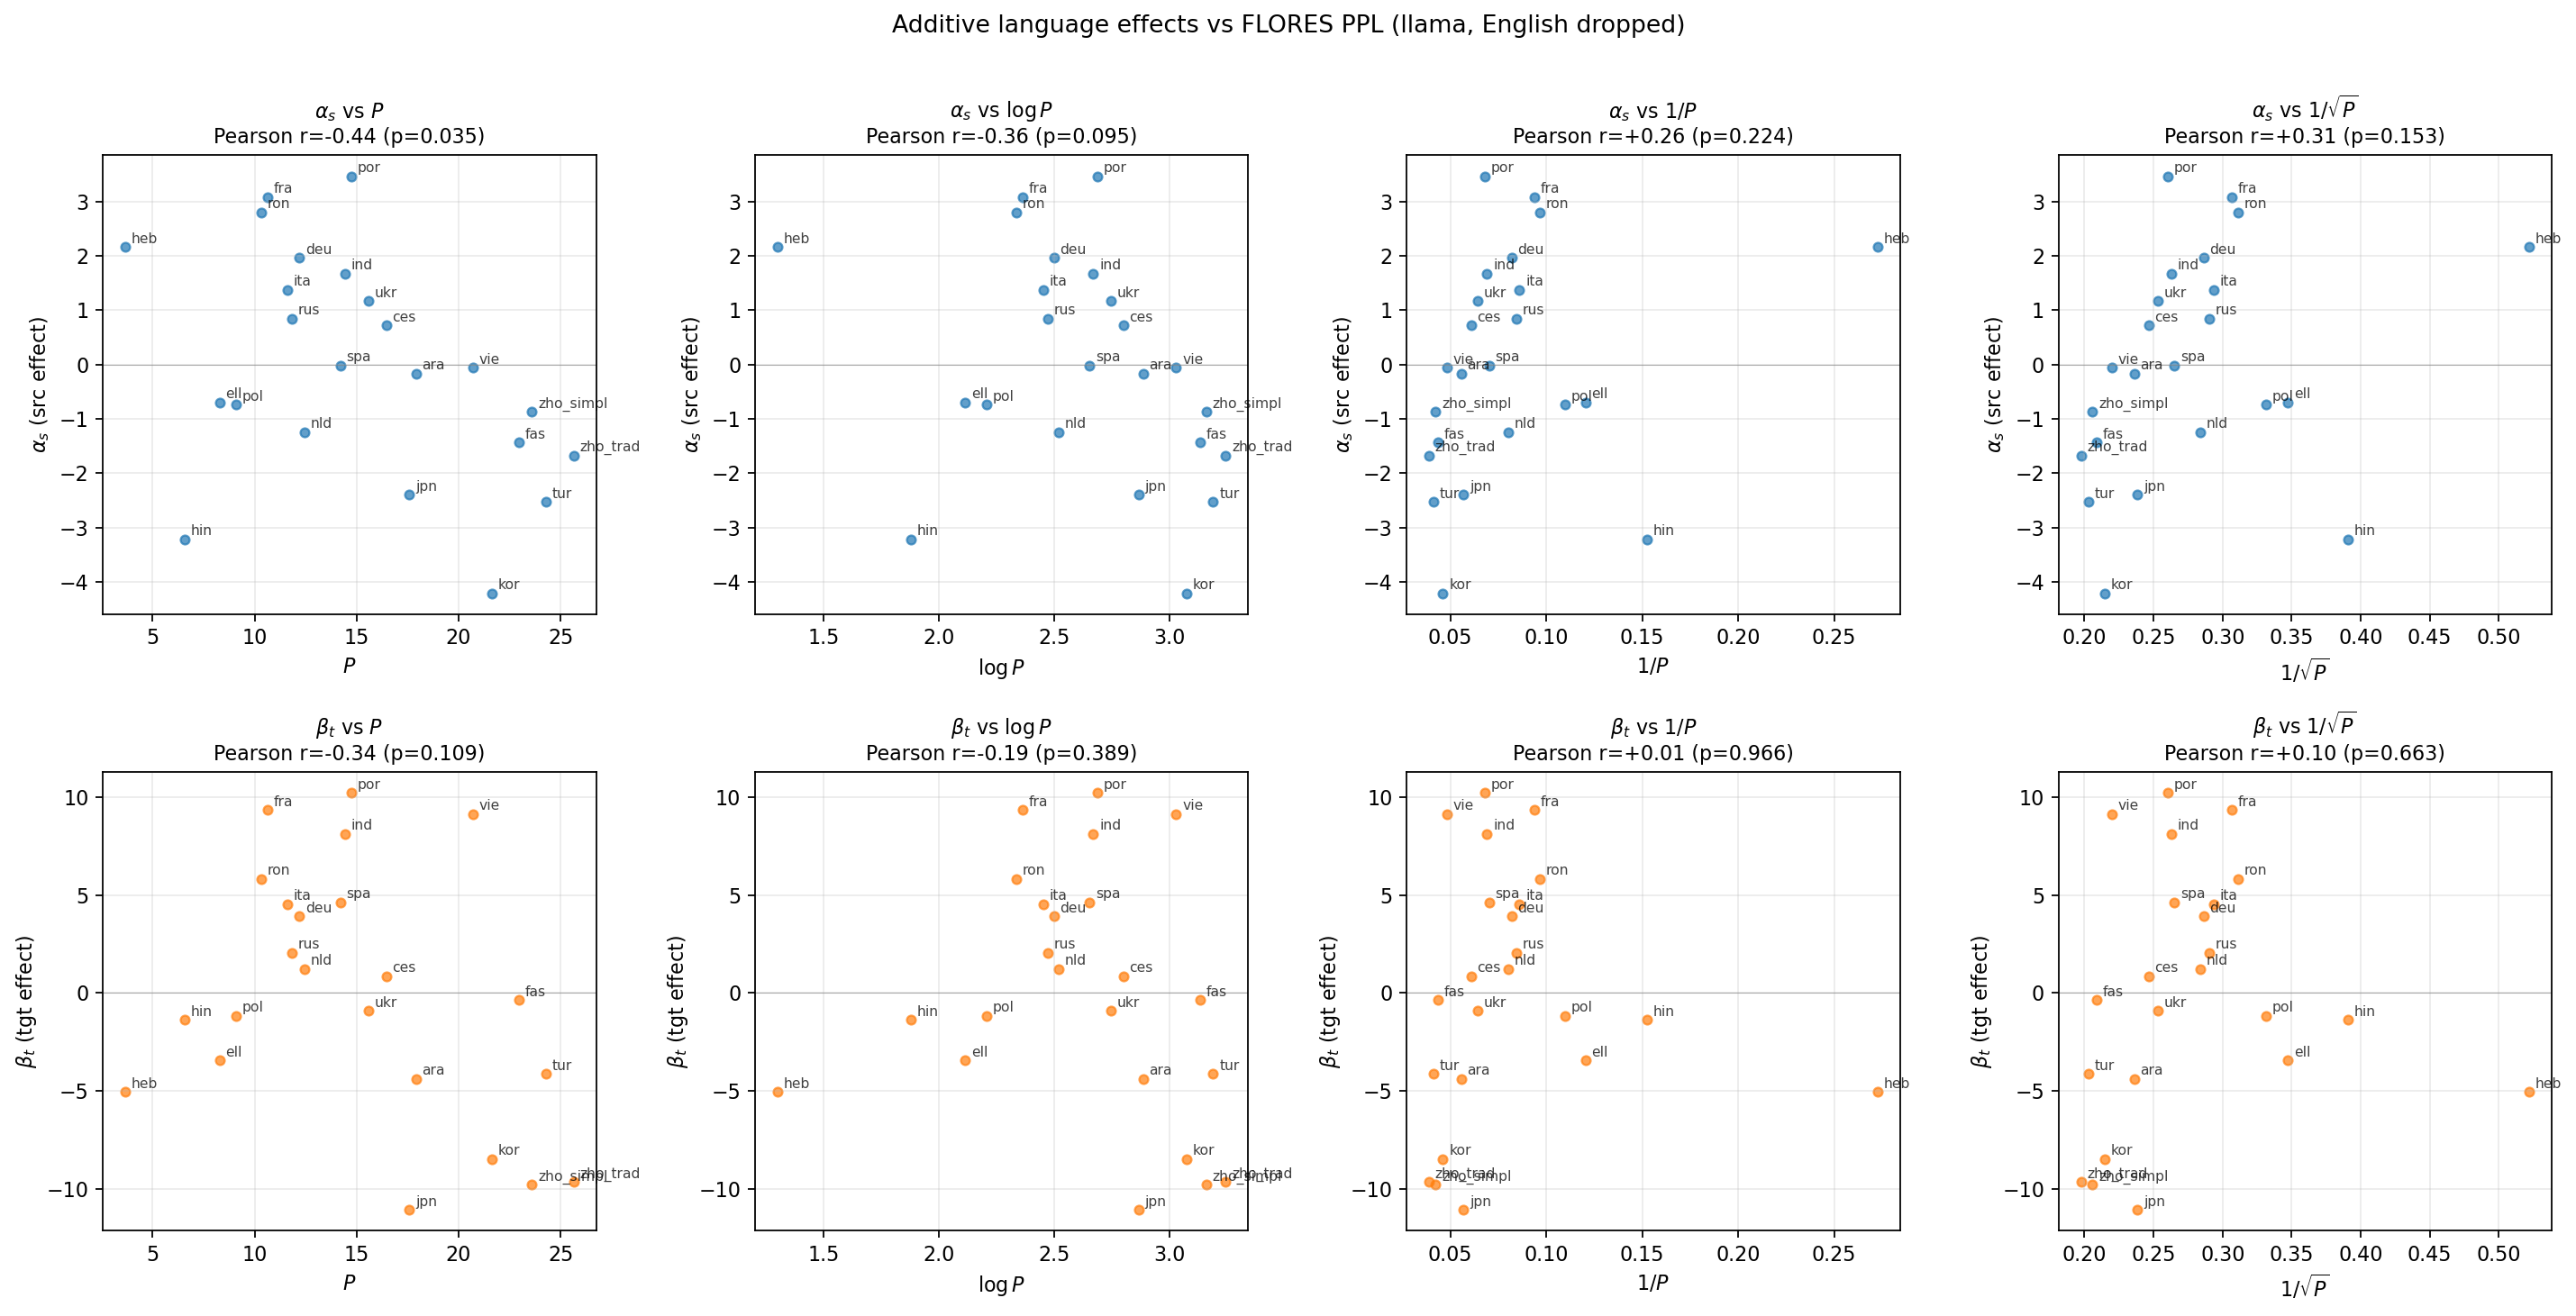
\includegraphics[width=0.95\linewidth]{../../img/perplexity_bleu_linear/alpha_beta_vs_ppl_no_eng_llama.png}
\caption{Llama (English removed): additive $\alpha_s$ and $\beta_t$ vs
FLORES PPL transforms. Without English's high-leverage point, the trend
across the remaining 23 languages is clearly visible.}
\end{figure}

\begin{figure}[h]
\centering
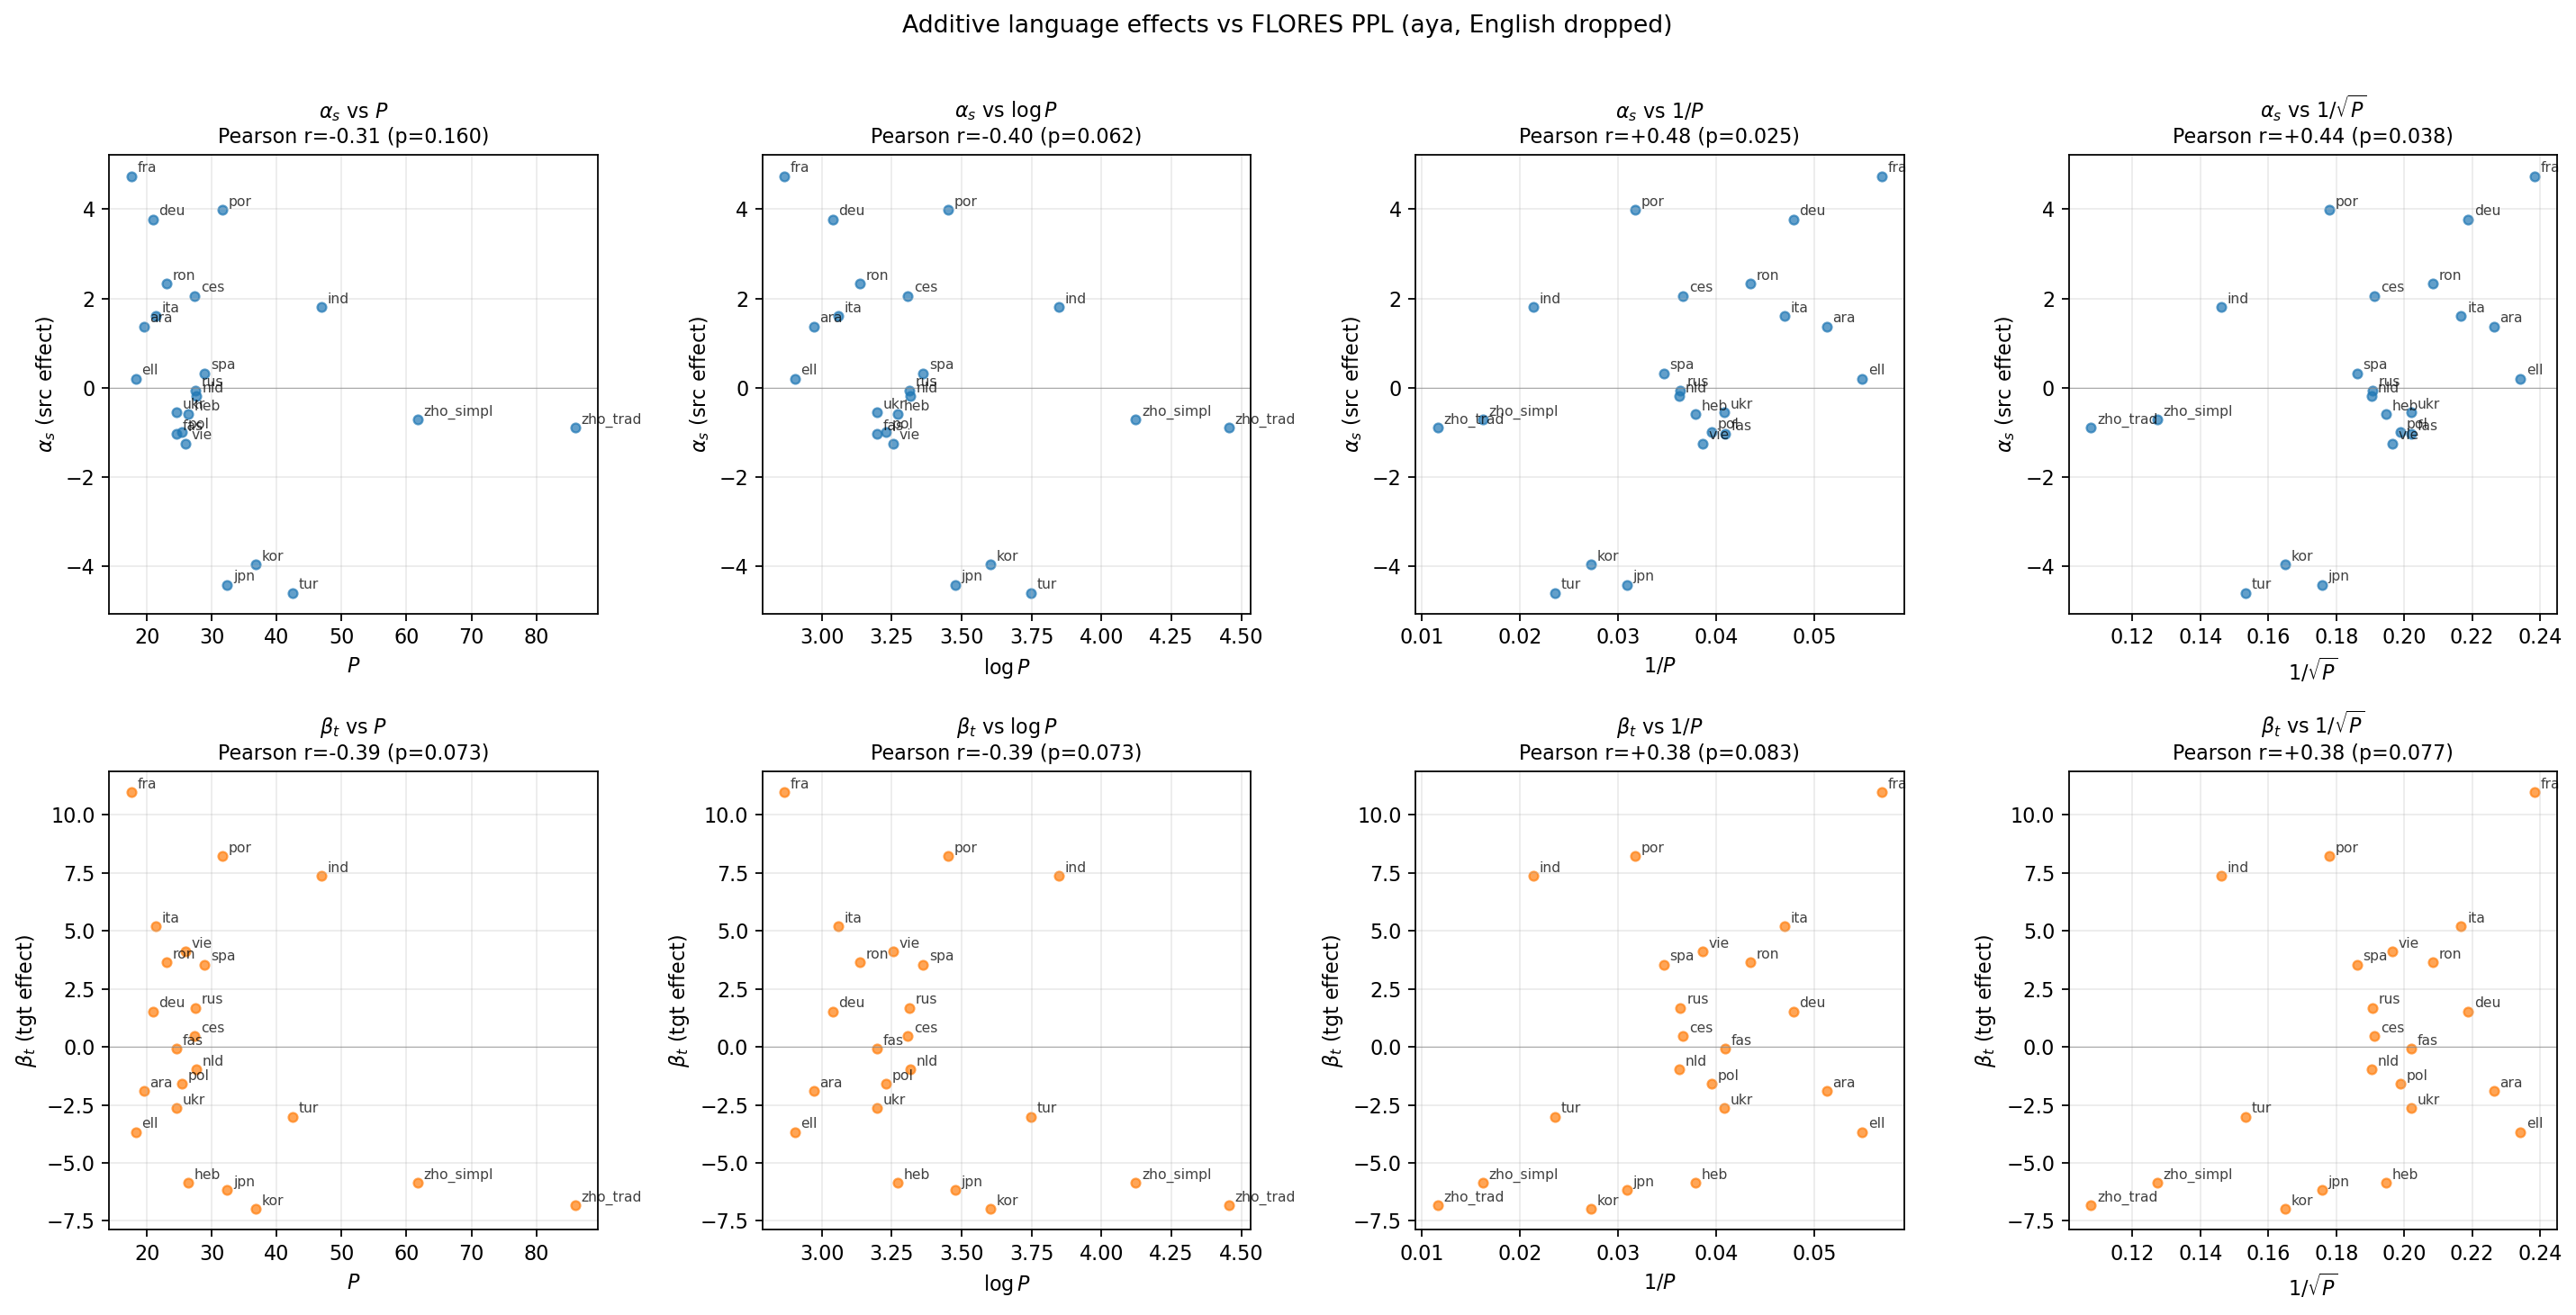
\includegraphics[width=0.95\linewidth]{../../img/perplexity_bleu_linear/alpha_beta_vs_ppl_no_eng_aya.png}
\caption{Aya (English removed): additive $\alpha_s$ and $\beta_t$ vs
FLORES PPL transforms.}
\end{figure}

\section{Experiment 9: Does the improved $\alpha,\beta$ vs PPL correlation
propagate to direct PPL $\to$ BLEU prediction?}

\subsection{Goal}

Experiment 8 showed that dropping English roughly doubles the Pearson
correlation between additive language effects ($\alpha, \beta$) and FLORES
PPL for Llama, and modestly tightens Aya's. Additive effects themselves
explain $\sim\!90\%$ of centered BLEU variance (Experiments~4/7). So if
PPL has decent correlation with $\alpha, \beta$ and $\alpha, \beta$
predict BLEU well, then direct PPL $\to$ BLEU regression should improve
too. This experiment tests that prediction.

\subsection{Method}

Repeat the regressions of Experiments~1 (BLEU $\sim P_s + P_t$, with and
without an interaction term) and Experiment~3 ($\log\code{bleu} \sim
\log P_s + \log P_t$), but on the no-English subset (n = 506 pairs per
model).

Also compute the \emph{chain-implied} $R^2$ from the additive
decomposition. For the additive matrix $\code{bleu}_{ij} \approx \mu +
\alpha_i + \beta_j$, the per-pair variance breaks into per-pair variance
of $\alpha$ + per-pair variance of $\beta$ (+ small residual). A linear
fit $\code{bleu} \sim f(P_s) + g(P_t)$ can therefore explain at most
\[
R^2_{\text{chain}} \approx r^2(\alpha, f(P)) \cdot
\frac{\mathrm{var}(\alpha_{\text{pair}})}{\mathrm{var}(\code{bleu})}
+ r^2(\beta, g(P)) \cdot
\frac{\mathrm{var}(\beta_{\text{pair}})}{\mathrm{var}(\code{bleu})},
\]
assuming $f(P_s)$ and $g(P_t)$ are uncorrelated across pairs (true here
by the full-grid design).

\subsection{Results}

\paragraph{Side-by-side: full (24-lang) vs no-eng (23-lang) BLEU $\sim$ PPL R²:}

\begin{center}
\small
\begin{tabular}{llrrr}
\toprule
model & form & $R^2$ full & $R^2$ no eng & $\Delta R^2$ \\
\midrule
aya   & $\code{bleu} \sim P_s + P_t$                    & 0.105 & 0.120 & $+0.015$ \\
aya   & $\code{bleu} \sim P_s + P_t + P_s \cdot P_t$    & 0.108 & 0.123 & $+0.016$ \\
aya   & $\log\code{bleu} \sim \log P_s + \log P_t$      & 0.136 & 0.145 & $+0.010$ \\
\midrule
llama & $\code{bleu} \sim P_s + P_t$                    & 0.021 & $\mathbf{0.114}$ & $\mathbf{+0.094}$ \\
llama & $\code{bleu} \sim P_s + P_t + P_s \cdot P_t$    & 0.021 & 0.116 & $+0.095$ \\
llama & $\log\code{bleu} \sim \log P_s + \log P_t$      & 0.042 & 0.082 & $+0.040$ \\
\bottomrule
\end{tabular}
\end{center}

\paragraph{Per-coefficient significance after dropping English:}

\begin{itemize}
  \item \textbf{Llama raw}: $P_s$ coef $p = 0.002$, $P_t$ coef $p = 2 \times
    10^{-13}$. Both highly significant; compare to full set where $P_s$ was
    n.s.\ ($p = 0.53$ on log scale, Exp~3).
  \item \textbf{Llama log}: $\log P_s$ $p = 0.20$ (still n.s.), $\log P_t$
    $p = 1 \times 10^{-10}$. Linear-in-$P$ is the better functional form for
    Llama after dropping English.
  \item \textbf{Aya raw}: $P_s$ $p = 0.005$, $P_t$ $p = 3 \times 10^{-13}$.
    Both highly significant.
  \item \textbf{Aya log}: $\log P_s$ $p = 7 \times 10^{-5}$, $\log P_t$
    $p = 8 \times 10^{-15}$. Both highly significant.
\end{itemize}

\paragraph{Interaction term:} Still not significant for either model under
either transform after dropping English ($p > 0.09$ everywhere). The
interaction term result from Experiment~1 is robust to outlier removal.

\paragraph{Chain-implied $R^2$ vs observed (raw transform):}

\begin{center}
\small
\begin{tabular}{lrrrrrrr}
\toprule
model & transform & $r^2(\alpha, f(P_s))$ & $r^2(\beta, g(P_t))$
      & $\mathrm{var}(\alpha_{\text{pair}})$ & $\mathrm{var}(\beta_{\text{pair}})$
      & $\mathrm{var}(\code{bleu})$ & $R^2_{\text{chain}}$ \\
\midrule
aya   & raw       & 0.096 & 0.152 & 5.97 & 25.25 & 35.63 & 0.124 \\
aya   & log       & 0.163 & 0.152 & 5.97 & 25.25 & 35.63 & 0.135 \\
aya   & $1/P$     & 0.227 & 0.143 & 5.97 & 25.25 & 35.63 & 0.139 \\
llama & raw       & 0.194 & 0.118 & 4.07 & 39.08 & 45.66 & 0.118 \\
llama & log       & 0.127 & 0.036 & 4.07 & 39.08 & 45.66 & 0.042 \\
llama & $1/P$     & 0.070 & 0.000 & 4.07 & 39.08 & 45.66 & 0.006 \\
\bottomrule
\end{tabular}
\end{center}

\paragraph{Observed vs predicted, raw form:}

\begin{center}
\small
\begin{tabular}{lrr}
\toprule
model & observed $R^2$ raw & chain-predicted $R^2$ raw \\
\midrule
aya   & 0.120 & 0.124 \\
llama & 0.114 & 0.118 \\
\bottomrule
\end{tabular}
\end{center}

The chain prediction matches the observed raw-form $R^2$ to within
$0.4$--$0.5$ percentage points for both models. The chain math holds
exactly.

\subsection{Interpretation}

\begin{enumerate}
  \item \textbf{The fit is no longer poor for Llama.} On the no-eng
    subset, the linear-in-raw-PPL model explains $R^2 = 0.114$ of BLEU
    variance --- a $5.5\times$ improvement over the full-set $R^2 = 0.021$.
    Both PPL coefficients are highly significant. The original
    ``$R^2 \approx 2\%$ Llama'' result was almost entirely an English
    outlier artifact.
  \item \textbf{The chain works as predicted.} The chain math
    ($R^2_{\text{chain}} = \sum r^2 \cdot \mathrm{var}/\mathrm{var}_{\text{BLEU}}$)
    predicts the observed raw-form fit to within $0.5$ pp for both
    models. There is nothing mysterious left to explain.
  \item \textbf{But the ceiling is still ~12--14\%, not 90\%.} Even with
    English removed and the chain saturating, $R^2$ is bounded by how well
    PPL predicts $\alpha, \beta$. With $r^2(\alpha, f(P)), r^2(\beta, g(P))
    \approx 0.13$--$0.16$ and $\alpha, \beta$ explaining $\sim 90\%$ of
    centered BLEU variance, the maximum reachable is
    $\sim 0.14$. Observed sits there. The remaining
    $\sim\!80$ pp gap from the additive ceiling is FLORES PPL being a
    genuinely noisy proxy for per-language competence --- not an
    overlooked outlier or wrong functional form.
  \item \textbf{Llama prefers raw-$P$ over $\log P$ now.} The chain
    table shows why: $r^2(\alpha, P_{\text{raw}}) = 0.194$ for Llama, vs
    $0.127$ for $\log P$. The English-induced inflation was hiding this
    --- on the full set $r$ was small for all transforms, so the choice
    didn't matter. Without English, raw $P$ tracks the rank-ordering of
    languages better than $\log P$ for Llama.
  \item \textbf{Aya barely moves.} As in Experiment~8, the Aya signal was
    already systematic. $R^2$ improves only $+1$--$2$ pp after dropping
    English.
\end{enumerate}

\paragraph{Synthesis with previous experiments.} The original Experiment~1
verdict (``linear-in-PPL barely works, interaction not significant'') was
substantially driven by Llama and substantially driven by English. Once
English is removed, linear-in-PPL works as well as the chain
$\text{PPL} \to \alpha, \beta \to \text{BLEU}$ allows. The interaction
term remains genuinely unimportant. So the H1-style story is:
\emph{BLEU is dominantly additive in per-language competence, and FLORES
PPL is a moderate-quality proxy for that competence in non-English
languages --- the linear-in-PPL fit captures most of what monolingual
PPL can capture}.

\paragraph{Outputs.}

\code{outputs/perplexity\_bleu\_linear/ppl\_to\_bleu\_no\_eng/observed\_fits.csv} \\
\code{outputs/perplexity\_bleu\_linear/ppl\_to\_bleu\_no\_eng/chain\_implied\_r2.csv} \\
\code{outputs/perplexity\_bleu\_linear/ppl\_to\_bleu\_no\_eng/comparison\_with\_full.csv}

\section{Experiment 10: Multi-BLiMP accuracy as the per-language proxy}
\label{sec:multiblimp}

\subsection{Goal}

The previous experiments characterized FLORES PPL as a noisy proxy for
per-language competence, with a chain ceiling of $R^2 \approx 0.14$ on
BLEU prediction (Experiment~9). Multi-BLiMP accuracy --- the proportion
of minimal pairs in the Multi-BLiMP grammatical-acceptability dataset
that the model scores correctly --- is a more direct measure of
per-language grammatical competence. We rerun Experiment~9's chain
analysis with Multi-BLiMP in place of PPL and ask whether it's a
stronger proxy.

\subsection{Important caveat: subset coverage}

Multi-BLiMP accuracy is available for only \textbf{17 of 24
languages}: \code{ces, deu, ell, eng, fas, fra, heb, hin, ita, nld,
pol, por, ron, rus, spa, tur, ukr}. The seven missing languages are
\code{ara, ind, jpn, kor, vie, zho\_simpl, zho\_trad} --- notably
including the major Llama outliers identified in Experiment~5
(\code{jpn}, \code{zho\_simpl}, \code{kor}).

For a fair PPL-vs-Multi-BLiMP comparison we fit \emph{both} predictors
on the same 17-language ($272$-pair) subset, and separately on the
no-English sub-subset ($16$-language, $240$-pair). This means the
Multi-BLiMP comparison runs on a subset that already filters out most
of the languages that hurt PPL most.

\subsection{Method}

For each subset (\code{full\_mbl}: $17$ langs; \code{no\_eng\_mbl}:
$16$ langs) and each model:

\begin{enumerate}
  \item Refit the additive RE model on this subset $\to$ new $\alpha,
    \beta$ for the chain math.
  \item Compute Pearson and Spearman correlations of $\alpha, \beta$
    against Multi-BLiMP accuracy under four transforms:
    \code{raw}~$= a$, \code{err}~$= 1 - a$, \code{log\_err}~$=
    \log(1 - a)$, \code{logit}~$= \log(a/(1-a))$.
  \item Fit $\code{bleu} \sim a_s + a_t$ (with and without
    interaction).
  \item Fit $\log\code{bleu} \sim \log(1 - a_s) + \log(1 - a_t)$
    (the log analog of Experiment~3's log-multiplicative form;
    $1 - a$ is the error rate, parallel to $P$).
  \item Same regressions with PPL on the same subset (baseline).
  \item Compute chain-implied $R^2$ for both predictors.
\end{enumerate}

\subsection{Additive RE on subset}

The additive fit stays strong on the smaller subsets:

\begin{center}
\small
\begin{tabular}{llrr}
\toprule
subset & model & $n$ langs & $R^2_{\text{additive,centered}}$ \\
\midrule
full\_mbl   & aya   & 17 & 0.912 \\
full\_mbl   & llama & 17 & 0.930 \\
no\_eng\_mbl & aya   & 16 & 0.891 \\
no\_eng\_mbl & llama & 16 & 0.901 \\
\bottomrule
\end{tabular}
\end{center}

So Section~\ref{sec:structural}'s ``BLEU is dominantly additive''
conclusion is unchanged on this subset. The chain ceiling is $\sim
90\%$, same as before.

\subsection{$\alpha, \beta$ vs Multi-BLiMP correlations}

\begin{table}[h]
\centering
\small
\begin{tabular}{lllrrrr|rrrr}
\toprule
 & & & \multicolumn{4}{c|}{full\_mbl ($n=17$)} & \multicolumn{4}{c}{no\_eng\_mbl ($n=16$)} \\
model & role & transform & Pearson $r$ & $p$ & Spearman $\rho$ & sig?\@ & Pearson $r$ & $p$ & Spearman $\rho$ & sig?\@ \\
\midrule
aya   & src & raw     & $+0.74$ & $0.001$ & $+0.72$ & $^{**}$ & $+0.75$ & $0.001$ & $+0.68$ & $^{**}$ \\
aya   & src & log\_err & $-0.82$ & $0.0001$ & $-0.72$ & $^{***}$ & $-0.77$ & $0.001$ & $-0.68$ & $^{**}$ \\
aya   & src & logit   & $+0.82$ & $0.0001$ & $+0.72$ & $^{***}$ & $+0.77$ & $0.001$ & $+0.68$ & $^{**}$ \\
aya   & tgt & raw     & $+0.63$ & $0.008$ & $+0.67$ & $^{**}$ & $+0.62$ & $0.014$ & $+0.62$ & $^{*}$ \\
aya   & tgt & log\_err & $-0.78$ & $0.0004$ & $-0.67$ & $^{***}$ & $-0.71$ & $0.003$ & $-0.62$ & $^{**}$ \\
aya   & tgt & logit   & $+0.77$ & $0.0005$ & $+0.67$ & $^{***}$ & $+0.70$ & $0.004$ & $+0.62$ & $^{**}$ \\
\midrule
llama & src & raw     & $+0.35$ & $0.16$ & $+0.31$ & --- & $+0.25$ & $0.35$ & $+0.13$ & --- \\
llama & src & log\_err & $-0.38$ & $0.13$ & $-0.31$ & --- & $-0.06$ & $0.84$ & $-0.13$ & --- \\
llama & tgt & raw     & $+0.54$ & $0.024$ & $+0.60$ & $^{*}$ & $+0.54$ & $0.031$ & $+0.51$ & $^{*}$ \\
llama & tgt & log\_err & $-0.65$ & $0.005$ & $-0.60$ & $^{**}$ & $-0.48$ & $0.063$ & $-0.51$ & --- \\
llama & tgt & logit   & $+0.64$ & $0.005$ & $+0.60$ & $^{**}$ & $+0.49$ & $0.057$ & $+0.51$ & --- \\
\bottomrule
\end{tabular}
\caption{Correlations of additive $\alpha, \beta$ with Multi-BLiMP
accuracy. $^{*}p<0.05$, $^{**}p<0.01$, $^{***}p<0.001$. Strong
significant correlations across the board for Aya; significant for
Llama tgt but weaker for Llama src.}
\end{table}

Compare to FLORES PPL correlations (Experiment~5) which topped out at
$|r| = 0.41$ for Aya src and $|r| = 0.36$ for Llama src on the full
24-lang set.

\subsection{BLEU $\sim$ Multi-BLiMP vs BLEU $\sim$ PPL fits}

\begin{table}[h]
\centering
\small
\begin{tabular}{llcc}
\toprule
subset & form & aya $R^2$ & llama $R^2$ \\
\midrule
\multirow{4}{*}{full\_mbl ($n=272$)}
 & $\code{bleu} \sim P_s + P_t$                              & 0.061 & 0.071 \\
 & $\log\code{bleu} \sim \log P_s + \log P_t$                & 0.068 & 0.128 \\
 & $\code{bleu} \sim a_s + a_t$                              & $\mathbf{0.394}$ & $\mathbf{0.250}$ \\
 & $\log\code{bleu} \sim \log(1-a_s) + \log(1-a_t)$          & $\mathbf{0.444}$ & $\mathbf{0.339}$ \\
\midrule
\multirow{4}{*}{no\_eng\_mbl ($n=240$)}
 & $\code{bleu} \sim P_s + P_t$                              & 0.130 & 0.009 \\
 & $\log\code{bleu} \sim \log P_s + \log P_t$                & 0.108 & 0.064 \\
 & $\code{bleu} \sim a_s + a_t$                              & $\mathbf{0.372}$ & $\mathbf{0.226}$ \\
 & $\log\code{bleu} \sim \log(1-a_s) + \log(1-a_t)$          & $\mathbf{0.358}$ & $\mathbf{0.194}$ \\
\bottomrule
\end{tabular}
\caption{Multi-BLiMP delivers $3$--$6\times$ the $R^2$ of FLORES PPL on
the same 17-language subset. Per-coefficient $p$-values for both PPL
and Multi-BLiMP coefs in these fits are typically $< 10^{-5}$;
interaction terms are not significant ($p > 0.4$).}
\end{table}

\subsection{Chain prediction vs observed (raw BLEU regressions)}

\begin{center}
\small
\begin{tabular}{llcc}
\toprule
subset & model & observed $R^2$ (BLEU $\sim a_s + a_t$) & chain-predicted $R^2$ \\
\midrule
full\_mbl    & aya   & 0.394 & 0.420 \\
full\_mbl    & llama & 0.250 & 0.259 \\
no\_eng\_mbl & aya   & 0.372 & 0.398 \\
no\_eng\_mbl & llama & 0.226 & 0.233 \\
\bottomrule
\end{tabular}
\end{center}

Chain prediction matches observed to within $1$--$3$ pp. The chain math
extends cleanly to Multi-BLiMP.

\subsection{Chain ceiling: what's possible with the best transform}

\begin{center}
\small
\begin{tabular}{llrrr}
\toprule
subset & model & best Multi-BLiMP $R^2_{\text{chain}}$ & best PPL $R^2_{\text{chain}}$ & MBL/PPL ratio \\
\midrule
full\_mbl    & aya   & 0.597 (log\_err) & 0.065 (raw) & $9.2\times$ \\
full\_mbl    & llama & 0.360 (log\_err) & 0.133 (inv) & $2.7\times$ \\
no\_eng\_mbl & aya   & 0.489 (log\_err) & 0.140 (log) & $3.5\times$ \\
no\_eng\_mbl & llama & 0.233 (raw)     & 0.106 (inv) & $2.2\times$ \\
\bottomrule
\end{tabular}
\caption{Best chain-implied $R^2$ ceiling per predictor and subset.
Multi-BLiMP gives substantially more headroom than PPL.}
\end{table}

\subsection{Interpretation}

\begin{enumerate}
  \item \textbf{Multi-BLiMP is a much stronger proxy for per-language
    competence than FLORES PPL.} On the same 17-lang subset, Multi-BLiMP
    delivers $R^2 = 0.39$--$0.44$ for Aya and $R^2 = 0.25$--$0.34$ for
    Llama, vs PPL's $R^2 = 0.06$--$0.13$. The chain ceiling jumps from
    $\sim\!14\%$ (PPL) to $\sim\!60\%$ (Aya) or $\sim\!36\%$ (Llama)
    --- a $3$--$9\times$ improvement.

  \item \textbf{Per-language correlations are dramatic for Aya.}
    $|r(\alpha, \text{logit}\,a_s)| = 0.82$ for Aya src and $0.77$ for
    Aya tgt --- both $p < 0.001$. These are the strongest per-language
    competence-vs-proxy correlations in the entire project.

  \item \textbf{Llama src is the weak point, even for Multi-BLiMP.}
    Llama's $\alpha$ (src effect) correlates only $|r| \approx 0.35$
    with Multi-BLiMP, vs $|r| = 0.54$--$0.65$ for $\beta$ (tgt
    effect). This is consistent with translation as src being more
    about \emph{content understanding} than \emph{grammatical
    knowledge of the src language} --- Multi-BLiMP measures the latter
    and underpredicts the former. Llama tgt, by contrast, is dominantly
    about generation in the target language, where grammatical
    competence directly applies.

  \item \textbf{Dropping English barely matters for Multi-BLiMP.}
    Unlike Experiment~8 (where dropping English roughly doubled Llama's
    PPL correlations), removing English from the Multi-BLiMP subset
    leaves $\alpha, \beta$ correlations essentially unchanged for Aya
    and slightly \emph{weakens} them for Llama. English is not an
    outlier in the Multi-BLiMP framework --- its high BLEU is
    consistent with its high Multi-BLiMP accuracy.

  \item \textbf{The chain math extends cleanly.} Observed raw-form $R^2$
    matches the chain prediction $\sum r^2 \cdot \mathrm{var} /
    \mathrm{var}_{\text{BLEU}}$ to within $1$--$3$ pp for both models
    and both subsets.

  \item \textbf{For Aya, $\log$/logit transforms substantially help; for
    Llama, raw is best.} The log\_err / logit transforms double Aya's
    chain $R^2$ (from $0.42$ raw to $0.60$ logit), reflecting the
    nonlinearity of the accuracy-to-competence relationship. Llama
    benefits less from log-style transforms.

  \item \textbf{What this means for H1.} The H1 hypothesis ``BLEU is
    predictable from monolingual competence'' is much more strongly
    supported by Multi-BLiMP than by FLORES PPL. The ``per-language
    competence latents'' that drive BLEU are well-captured by an
    acceptability-based grammatical measure ($|r|$ up to $0.82$), and
    that translates directly into predictive power ($R^2$ up to $0.44$
    observed, $0.60$ chain-ceiling). FLORES corpus PPL is, by
    comparison, a substantially noisier proxy --- it confounds
    grammatical knowledge with topical / lexical familiarity that's
    less directly tied to translation BLEU.
\end{enumerate}

\paragraph{Outputs.}

\code{outputs/perplexity\_bleu\_linear/bleu\_to\_multiblimp/observed\_fits.csv} \\
\code{outputs/perplexity\_bleu\_linear/bleu\_to\_multiblimp/alpha\_beta\_vs\_mbl.csv} \\
\code{outputs/perplexity\_bleu\_linear/bleu\_to\_multiblimp/chain\_implied\_r2.csv} \\
\code{outputs/perplexity\_bleu\_linear/bleu\_to\_multiblimp/additive\_re\_on\_subset.csv}

\section{Status after Experiments 1--10}

The picture is much sharper now:

\begin{itemize}
  \item BLEU's per-language structure is \textbf{dominantly additive}.
    On the like-for-like comparison (Section~\ref{sec:structural}),
    additive explains $0.932 / 0.879$ of centered BLEU variance vs
    $0.859 / 0.716$ for the structurally-comparable multiplicative model.
    AMMI shows only $+3$--$5$ pp of genuinely multiplicative residual
    interaction. The original ``rank-1 $\approx 88\%$'' was on an
    uncentered Frobenius scale inflated by the grand mean.
  \item \textbf{The choice of proxy matters more than the functional
    form.} On the same 17-language subset, Multi-BLiMP accuracy delivers
    $R^2 = 0.39$--$0.44$ (Aya) and $R^2 = 0.25$--$0.34$ (Llama) for
    direct BLEU prediction. FLORES PPL on the same subset achieves only
    $R^2 = 0.06$--$0.13$. Multi-BLiMP is a $3$--$6\times$ stronger
    per-language competence proxy (Experiment~10), pushing the chain
    ceiling from $\sim 14\%$ (PPL) to $\sim 36$--$60\%$ (Multi-BLiMP).
  \item \textbf{Per-language correlations approach $|r| = 0.82$ with
    Multi-BLiMP} (Aya src, logit transform). This is the strongest
    per-language competence-vs-proxy correlation in the project.
    English is not an outlier in the Multi-BLiMP framework --- its high
    BLEU is consistent with its high Multi-BLiMP accuracy.
  \item FLORES PPL is a \textbf{moderate, systematic} proxy for those
    additive effects on non-English languages: $|r| \approx
    0.35$--$0.45$ after dropping English (Experiment~8). English is
    high-leverage for the PPL story (halves Llama's correlations on the
    full set) but not for the Multi-BLiMP story.
  \item The direct \textbf{linear-in-PPL fit works as predicted by the
    chain math} once English is removed: Llama goes from $R^2 = 0.02
    \to 0.11$ (Experiment~9). Observed $R^2$ matches the chain
    prediction $\sum r^2 \cdot \mathrm{var}/\mathrm{var}_{\text{BLEU}}$
    to within $0.5$ pp for raw transforms, both for PPL and
    Multi-BLiMP.
  \item The interaction term remains \textbf{not significant} for any
    predictor / transform / subset combination tested. The
    Experiment~1 result is robust.
  \item \textbf{Llama src is the weak point}, even with Multi-BLiMP
    ($|r(\alpha, \text{logit}\,a) | \approx 0.38$ vs $0.65$ for tgt).
    Translation as source is plausibly more about content understanding
    than about grammatical knowledge of the source language;
    Multi-BLiMP measures the latter and underpredicts the former.
  \item The src/tgt asymmetry across Experiments 2/5 vs Experiment 3 is
    fully explained: the BLEU matrix is much more tgt-driven than
    src-driven (variance ratio $4$--$9\times$), but src has the
    cleaner per-language rank-ordering by either proxy.
\end{itemize}

Natural next moves: (a) extend Multi-BLiMP coverage to the missing
languages (currently \code{ara, ind, jpn, kor, vie, zho\_*}) to test
whether the Multi-BLiMP advantage scales to the full BLEU matrix;
(b) construct a hybrid proxy combining Multi-BLiMP (grammatical
competence) with a content-understanding measure (FLORES PPL?
NLI accuracy?) to close the Llama src gap; (c) repeat the drop-language
ablations for CJK targets in the PPL framework, now as a sanity check
rather than primary analysis.

\end{document}
